\documentclass{article}

%-------Packages---------
\usepackage[utf8]{inputenc}
\usepackage[margin=1.5in]{geometry}
\usepackage{amssymb,amsmath,amsfonts,amsthm}
\usepackage{enumerate}
\usepackage{mathrsfs}
\usepackage[ruled,vlined]{algorithm2e}
\usepackage{graphicx}
\usepackage{titling}
\usepackage{subcaption}
\captionsetup[subfigure]{labelfont=rm}

\numberwithin{equation}{section}
\newcommand{\code}[1]{\text{{\fontfamily{lmtt}\selectfont #1}}}

\bibliographystyle{unsrt}

%--------Theorem Environments--------
%theoremstyle{plain} --- default
\theoremstyle{definition}
\newtheorem{thm}{Theorem}[section]
\newtheorem{cor}[thm]{Corollary}
\newtheorem{prop}[thm]{Proposition}
\newtheorem{lem}[thm]{Lemma}
\newtheorem{conj}[thm]{Conjecture}
\newtheorem{quest}[thm]{Question}

% \newtheoremstyle{definition}
\newtheorem{defn}[thm]{Definition}
\newtheorem{defns}[thm]{Definitions}
\newtheorem{con}[thm]{Construction}
\newtheorem{exmp}[thm]{Example}
\newtheorem{exmps}[thm]{Examples}
\newtheorem{notn}[thm]{Notation}
\newtheorem{notns}[thm]{Notations}
\newtheorem{addm}[thm]{Addendum}
\newtheorem{exer}[thm]{Exercise}

% \newtheoremstyle{remark}
\newtheorem{rem}[thm]{Remark}
\newtheorem{rems}[thm]{Remarks}
\newtheorem{warn}[thm]{Warning}
\newtheorem{sch}[thm]{Scholium}

%--------Meta Data: Fill in your info------
% Sharon Zhang
% Advised by Prof. Nicolas Boumal, Dr. Amit Moscovich
% Princeton University
% Dept. of Mathematics

\title{\textbf{Analyzing product manifolds using \\ diffusion maps}}

\author{Sharon Zhang \\ \vspace{1.0mm} \\ Advised by: \\ Professor Nicolas Boumal and Dr. Amit Moscovich}

\date{}

\begin{document}
\begin{titlepage}
    \clearpage\maketitle
    \thispagestyle{empty}
   \begin{center}
      
        Junior Paper\\
        Department of Mathematics\\
       Princeton University
       
       \vspace{0.5cm}
      
\includegraphics[width=0.1\textwidth]{images/university.png}
        \vspace{0.35cm}
       
       \textit{This paper represents my own work in accordance \\ with University regulations.}
       /s/ Sharon Zhang \\
       
       \vspace{0.35cm}
         May 15, 2020
       
        \vfill

        \begin{abstract}
        Diffusion maps are a spectral method for dimensionality reduction which exploit the intrinsic geometry of data. Given a set of points sampled from a manifold, the eigenvectors of the diffusion map formed by those samples are discrete approximations of the Laplace eigenfunctions of the manifold. Using this relationship, we propose an algorithm for decomposing product manifolds into independent submanifolds and test it on simulated data sampled from submanifolds of $\mathbb{R}^D$. Our results show that the algorithm performs well on these manifolds, and can potentially be adapted for applications such as single-particle reconstruction in cryo-electron microscopy.
        \end{abstract}
   \end{center}
\end{titlepage}

\tableofcontents
\newpage

\section{Introduction}
Suppose we have some data $\textbf{x}_1, \ldots, \textbf{x}_n$ which are independent identically distributed samples from a distribution over the manifold $\mathcal{M} \subset \mathbb{R}^D$. The $D$ dimensions encode information about all variables present in our data, but it is possible that there is no correlation between many of these variables. For example, we may know $\mathcal{M} = \mathcal{M}_1 \times \mathcal{M}_2$, where $\dim\mathcal{M} = d \le D$ and
\[
d = d_1+d_2 = \dim\mathcal{M}_1 + \dim\mathcal{M}_2
\]
and $\mathcal{M}_1$, $\mathcal{M}_2$ describe independent variables. Our observations of $\{\textbf{x}_i\}_{i=1}^n$ lie in the ambient space $\mathbb{R}^D$, but it is desirable to analyze these samples in $\mathcal{M}_1$ and $\mathcal{M}_2$ separately rather than in $\mathcal{M}$ or $\mathbb{R}^D$. Additionally, we may also want to recover the geometry of $\mathcal{M}_1$ and $\mathcal{M}_2$, so that we can learn more information about the variables which they represent. In particular, one important instance of this problem arises in cryogenic-electron microscopy.

\subsection{Cryogenic-electron microscopy}
\begin{figure}
    \centering
    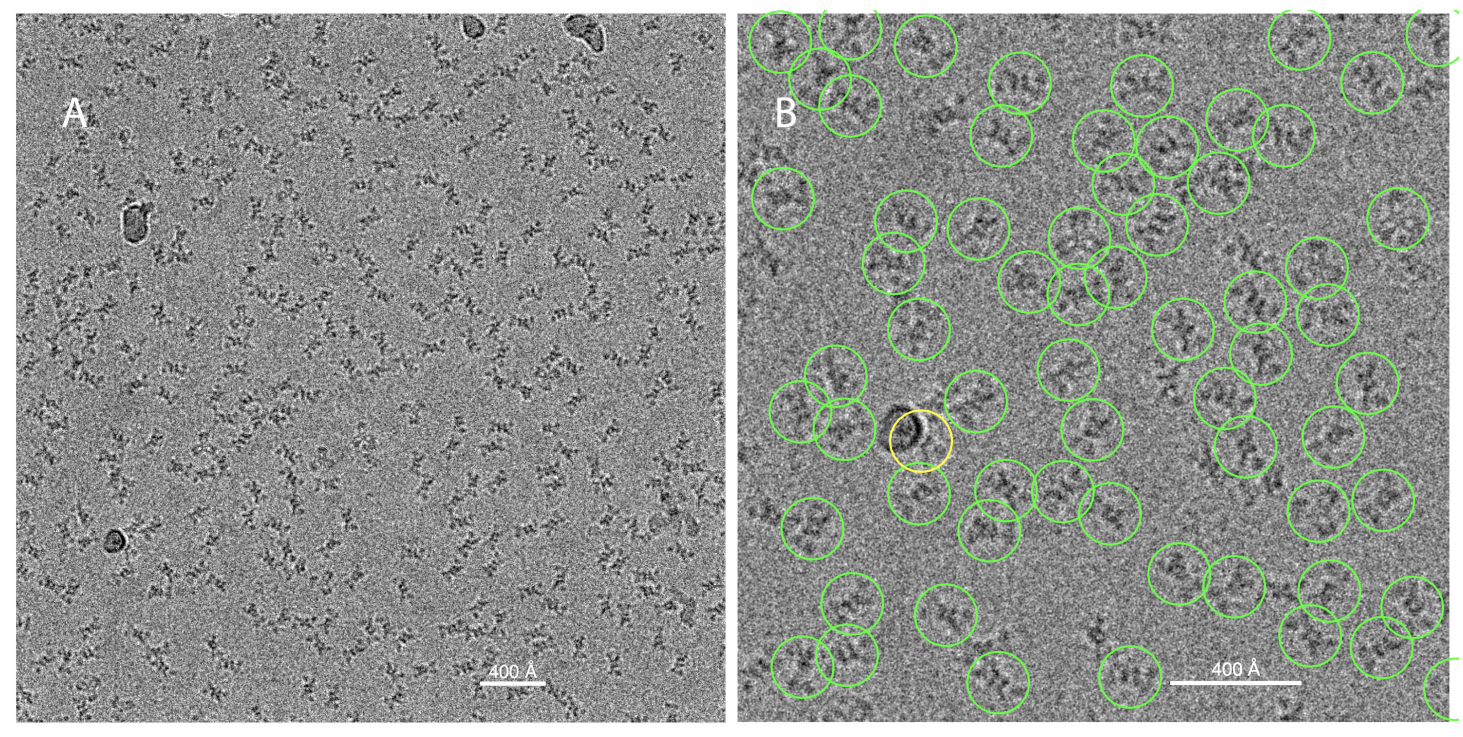
\includegraphics[width=\textwidth]{images/cryo-em.png}
    \caption{(Left) A cryo-EM micrograph of PaaZ protein particles obtained using a Titan Krios microscope, displayed after applying a low-pass filter for clarity. (Right) A close-up of the micrograph, with PaaZ particles identified in green. The images are by Singer and Sigworth \cite{SingerSigworth2020}.}
    \label{fig:cryo-em}
\end{figure}
Cryogenic-electron microscopy (cryo-EM) is a technique commonly used in biology for imaging molecules. Before an image is taken, samples are frozen at cryogenic temperatures, enabling them to be captured in their natural environment. The frozen particles are then visualized using an electron microscope to produce a \textit{micrograph} (see Figure \ref{fig:cryo-em}), which contains many instances of image patches with molecules \cite{Frank_2006}. The images produced by cryo-EM are two-dimensional tomographic projections of the particle's electrostatic potential \cite{Vulovi__2013}. One goal of collecting these two-dimensional images is to create a three-dimensional reconstruction of the particle.

Due to the low signal-to-noise (SNR) ratio of these micrographs \cite{singer2018mathematics}, many images of identical molecules are required in order to reconstruct a single molecule. During the freezing process, the molecules are trapped in a random position and orientation. Thus the resulting image data for a single molecule is not necessarily consistent across images. One important variable is the inherent orientation of the particular molecule, which is a primary factor influencing these inconsistent appearances. 

\subsection{The classic reconstruction problem}
We can model the entire electrostatic potential of the particle as a function $\phi : \mathbb{R}^3 \rightarrow \mathbb{R}$. As described in \cite{singer2018mathematics}, an image $I$ of a molecule is obtained from $\phi$ by:
\begin{enumerate}[(i)]
    \item applying a rotation $R$;
    \item projecting in the $z$-direction;
    \item convolving with a point-spread function $H$;
    \item sampling on an $L \times L$ Cartesian grid of pixels;
    \item and adding noise.
\end{enumerate}
Formally, we can write the final image as
\begin{equation}
    I(x,y) = H \star PR \circ \phi + \omega 
\end{equation}
where $P$ is the tomographic projection operator in the $z$-direction, $P f(x,y) = \int_{-\infty}^\infty f(x,y,z) dz$, and $R \circ \phi = \phi(R^T r)$, $r = (x,y,z)^T$. The classic cryo-EM reconstruction problem is posed as follows: given $n$ images $I_1, \ldots I_n$ and the corresponding point spread functions $H_1, \ldots, H_n$, how can we recover $\phi$ without knowing $R_1, \ldots, R_n$?\footnote{A simple extension of this classical reconstruction problem is to assume \textit{discrete heterogeneity}, in which we assume that $\{\phi_i\}_{i=1}^n$ come from a small fixed set of conformations.}

\subsection{The heterogeneity reconstruction problem}
\begin{figure}
    \centering
    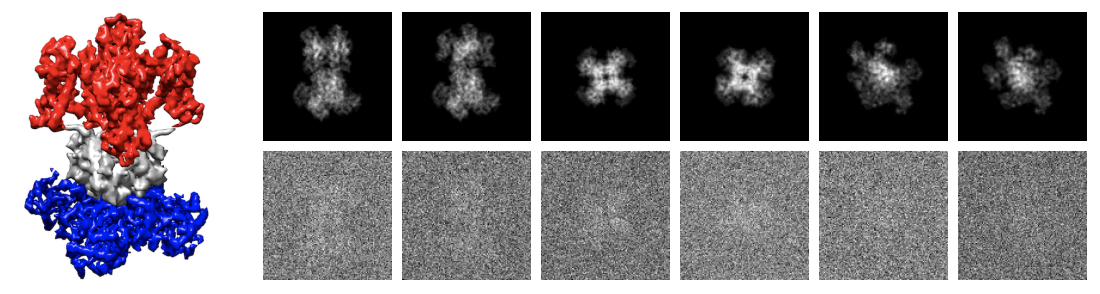
\includegraphics[width=\textwidth]{images/heterogeneity-problem.png}
    \caption{(Left) A potassium ion channel with two deformable parts. The red portion of the molecule is randomly rotated around the $z$-axis, and the blue portion of the molecule is stretched along the $xy$-plane. (Right) Two different conformations of the molecule, projected in three different orientations (top view, side view, oblique view). The images along the top row are clean, whereas the images along the bottom row have added noise. The figure is originally by Moscovich et al \cite{MoscovichHaleviAndenSinger2020}.}
    \label{fig:heterogeneity}
\end{figure}

An even harder problem is known as the \textit{heterogeneity} cryo-EM problem. The challenge in this variation arises from potential structural variations within the molecules \cite{singer2018mathematics, MoscovichHaleviAndenSinger2020}. Namely, for different images $I_i$ we may potentially capture different molecular conformations $\phi_1, \ldots, \phi_n$. An example of this is illustrated in Figure \ref{fig:heterogeneity}. The heterogeneity cryo-EM problem requires restrictive assumptions in order to ensure that the number of output parameters in $\{\phi_i\}_{i=1}^n$ can be solved for using the number of input parameters given by $\{I_i\}_{i=1}^n$, $\{H_i\}_{i=1}^n$. One reasonable assumption is that the variability of the conformations $\{\phi_i\}_{i=1}^n$ is continuous, and thus we are able to model the conformations by a manifold \cite{MoscovichHaleviAndenSinger2020}.

In this paper, we propose an algorithm to isolate the submanifolds from an ambient product manifold, inspired by spectral analysis methods \cite{coifman2006diffusion, 10.5555/2980539.2980616, Belkin_2003} and prior work applying these techniques \cite{Singer_2006, zelesko2019earthmover}. We first provide a brief exposition of diffusion maps and the Laplacian operator, then we describe the algorithm, and finally we present the results of our method on some simulated data.

\section{Theory}
We begin by reviewing the definitions of the continuous Laplacian, as well as a few of its properties. We then examine how the Laplacian decomposes over product submanifolds of $\mathbb{R}^D$. Lastly, we go over results which relate the discrete Laplacian to the continuous Laplacian, and some spectral techniques for data analysis which make use of all these results.

\subsection{The Laplace operator}
Let $f : \mathbb{R}^n \rightarrow \mathbb{R}$ be a twice-differentiable function in Euclidean space. The Laplacian (or ``Laplace operator"), denoted by $\Delta$, is the differential operator

\begin{equation}\label{laplace}
    \Delta f = \nabla \cdot \nabla f = \sum_{i=1}^n \frac{\partial f}{\partial x^2_i}
\end{equation}
where $\nabla \cdot$ is the divergence operator and $\nabla f$ is the gradient of $f$. Informally, the Laplacian can be interpreted as a measure of the density of gradient flow at a certain point. As such, it is the backbone of many important physical equations, such as Poisson's Equation, which relates the electric potential to the electric charge density of a medium, and the wave equation, which describes the propagation of oscillations.

The \textit{spectrum} of the Laplacian is defined as the set of eigenvalues and associated eigenfunctions which satisfy the Helmholtz equation,
\begin{equation}\label{helmholtz}
    -\Delta f = \lambda f,
\end{equation}
also known as the ``Laplace eigenproblem". In particular, the Helmholtz equation on an interval $[a,b]$ can be posed as a Sturm-Liouville problem, which is of the form

\begin{equation}\label{S-L}
(p(x)y')' + q(x)y + \lambda w(x)y = 0
\end{equation}
with boundary conditions
\begin{align}\label{S-L-boundary}
    \alpha_1 y(a) + \alpha_2 y'(a) = 0, &\quad \alpha^2_1 + \alpha^2_2 > 0 \\
    \beta_1 y(b) + \beta_2 y'(b) = 0, &\quad \beta^2_1 + \beta^2_2 > 0.
\end{align}
One of the main results in Sturm-Liouville theory is the following theorem.

\begin{thm}\label{SL-theory}
If $p', q, w \in C([a,b])$ and $p(x), w(x) > 0$, then the Sturm-Liouville problem has an infinite set of solutions $\{f_i\}_{i=1}^\infty$ with eigenvalues
\begin{equation}\label{laplace-eigenvalues}
    0 = \lambda_1 \le \lambda_2 \le \ldots \rightarrow \infty.
\end{equation}
Moreover, these functions form an orthonormal basis of $L^2([a,b])$.
\end{thm}

\begin{proof}
See Chapter 2, Section 2.4 and Theorem 2.29 of \cite{sl-textbook}.
\end{proof}

\begin{rem}\label{spectral-thm}
The results of Theorem \ref{SL-theory} also apply to the solutions of the Helmholtz equation on a bounded Euclidean region $\Omega \subset \mathbb{R}^D$. That is, the eigenfunctions over $\Omega$ form an orthonormal basis of $L^2(\Omega)$. This follows from the Spectral Theorem on compact operators. For more detailed background, refer to Theorem 0.44 and the sections leading up to Theorem 7.28 of \cite{FOLLAND_2020}.
\end{rem}

The functions $\{f_i\}_{i=1}^\infty$ are known as the Laplace eigenfunctions of the manifold, and they are nice to work with because they are infinitely differentiable over the manifold interior (see Theorem 6 in Chapter 6, Section 6.3 of \cite{Evans_2010}). The following examples derive the Laplace eigenfunctions over some basic Euclidean regions.

\begin{exmp}[A line]\label{laplace-line}
Consider the Laplace eigenproblem over the line $\ell = [0,a]$,
\begin{equation}\label{line-problem}
\Delta u + \lambda u = u'' + \lambda u = 0, \quad 0 < x < a
\end{equation}
with Neumann boundary conditions
\begin{equation}\label{line-boundaries}
u'(0) = u'(a) = 0.
\end{equation}

Both $u(x) = \cos(\alpha x)$ and $u(x) = \sin(\alpha x)$ are solutions to (\ref{line-problem}). By (\ref{line-boundaries}), we can eliminate $\sin(\alpha x)$. Furthermore, we must have
\begin{equation}
    -\alpha \sin(\alpha a) = 0
\end{equation}
so $\alpha a = k\pi$ for some integer $k$. Then $\alpha = \frac{k\pi}{a}$, so our eigenfunctions are
\begin{equation}
    \cos\Big(\frac{k\pi}{a} x\Big), \quad k = 0, 1, 2, \ldots
\end{equation}
with eigenvalues
\begin{equation}
    \lambda_k = \frac{k^2\pi^2}{a^2}. 
\end{equation}
\end{exmp}

\begin{exmp}[A disk]\label{laplace-disk}
Let $\Omega$ be a disk with radius $R$. We reparametrize the Laplacian using polar coordinates
\begin{equation}
    r = \sqrt{x^2+y^2}, \quad \theta = \tan^{-1}\Big(\frac{y}{x}\Big)
\end{equation}
to get
\begin{equation}\label{circle-problem}
u_{rr} + \frac{1}{r}u_r + \frac{1}{r^2}u_{\theta\theta} + \lambda u = 0, \quad 0 \le r < R
\end{equation}
with Neumann boundary conditions
\begin{equation}\label{circle-boundaries}
u_r(r,\theta) = 0 \text{ at } r = R.
\end{equation}

A natural starting point is separation of variables, as we have two independent variables $r$ and $\theta$. This gives us $u(r,\theta) = R(r)\Theta(\theta)$, so
\begin{equation}
    R''\Theta + \frac{R'}{r}\Theta + \frac{R}{r^2}\Theta'' + \lambda R\Theta = 0.
\end{equation}
We can collect variables to get
\begin{equation}\label{separations}
    r^2\frac{R''}{R} + r\frac{R'}{R} + \lambda r^2 = -\frac{\Theta ''}{\Theta} = \alpha^2.
\end{equation}
Importantly, the left hand side depends only on $r$ and the right hand side depends only on $\theta$, so they must both be constant. We show later why this constant must be negative. The solutions to the $\Theta$ side of (\ref{separations}) are of the form
\begin{equation}
    A_k\cos(k\theta)+B_k\sin(k\theta).
\end{equation}
There are no boundary conditions on $\Theta$, but we must also have
\begin{align}
    A_k\cos(k\theta)+B_k\sin(k\theta) &= A_k\cos(k(\theta + 2m\pi))+B_k\sin(k(\theta + 2m\pi)) \\
    &= A_k\cos(k\theta + 2km\pi)+B_k\sin(k\theta + 2km\pi)
\end{align}
so $k$ must be an integer. Thus the solutions for $\Theta$ are
\begin{equation}\label{theta-sols}
    \Theta_k(\theta) = A_k\cos(k\theta)+B_k\sin(k\theta), \quad k= 0, 1, 2, \ldots
\end{equation}
The right hand side of the equation can be rewritten as
\begin{equation}\label{final-R}
    r^2R'' + rR' + (\lambda r^2 - \alpha^2)R = 0.
\end{equation}
Next, we substitute $R(r) = J(\sqrt{\lambda}r)$, which has the effect of rescaling $r$. This gives us
\begin{align}
    &R(r) = J(\sqrt{\lambda} r) \\
    &R'(r) = \sqrt{\lambda}J'(\sqrt{\lambda}r) \\
    &R''(r) = \lambda J''(\sqrt{\lambda}r)
\end{align}
Then (\ref{final-R}) becomes
\begin{equation}
    \lambda r^2 J''(\sqrt{\lambda}r) + \sqrt{\lambda}rJ'(\sqrt{\lambda}r) + (\lambda r^2 - \alpha^2)J(\sqrt{\lambda}r) = 0.
\end{equation}
We can also substitute $\beta = \sqrt{\lambda}r$, so (\ref{final-R}) becomes
\begin{equation}\label{bessels}
    \beta^2 J''(\sqrt{\lambda}r) + \beta rJ'(\sqrt{\lambda}r) + (\beta^2 - \alpha^2)J(\sqrt{\lambda}r) = 0.
\end{equation}
The above is known as Bessel's equation. The solutions to Bessel's equation with the imposed Neumann boundary conditions are the $k$th Bessel functions of the first-kind,
\begin{equation}\label{k-bessels}
    J_k(x) = \sum_{\ell=0}^\infty \frac{(-1)^\ell}{\ell!(k+\ell)!}\Big(\frac{x}{2}\Big)^{k+2\ell}
\end{equation}
with $J'_k(\sqrt{\lambda}r) = 0$. Combining (\ref{theta-sols}) with (\ref{k-bessels}), we get our eigenfunctions
\begin{equation}\label{disk-sols}
u(r,\theta) = \Theta_k(\theta)J_k(\sqrt{\lambda}r).
\end{equation}

It remains to be shown that the constant in (\ref{separations}) must be negative. First, suppose that it is equal to zero. Then we have $X'' = 0$, so $X$ is linear. By the boundary conditions, we must have $X = 0$, and hence $u = 0$. Next, consider the case in which the constant is positive. Then we must have $X'' = \alpha^2X$, which gives us the solutions $X(x) = A\cosh(\alpha x) + B\sinh(\alpha x)$. The boundary condition $X'(0) = 0$ implies $0 = A\sinh(0) + B\cosh(0) = (A + B)/2$, so $A = -B$. Substituting this into the other boundary condition gives us $X'(a) = A\sinh(\alpha a) - A\cosh(\alpha a) = 0$, so $\sinh(\alpha a) = \cosh(\alpha a)$. This requires $e^{-\alpha x} = 0$, which is impossible. Thus the constant must be positive.
\end{exmp}

\subsection{The Laplace operator over product spaces}
Suppose we have a manifold $\mathcal{M} = \mathcal{M}_1 \times \mathcal{M}_2$ in $\mathbb{R}^D$. To analyze $\mathcal{M}_1$ and $\mathcal{M}_2$, we would also like to look at the Laplace operator over these two regions separately. 

\begin{prop}\label{laplace-sum-decomp}
Let $\mathcal{M} = \mathcal{M}_1 \times \mathcal{M}_2$ be a product manifold in $\mathbb{R}^D$, such that $\dim\mathcal{M} = d \le D$. Then $\Delta_\mathcal{M} = \Delta_{\mathcal{M}_1} + \Delta_{\mathcal{M}_2}$.
\end{prop}
\begin{proof}
Write $d = d_1+d_2$ where $d_1 = \dim\mathcal{M}_1$ and $d_2 = \dim\mathcal{M}_2$. We have
\begin{equation}
\Delta_{\mathcal{M}} = \sum_{i=1}^d \frac{\partial}{\partial x_i} = \sum_{i=1}^{d_1} \frac{\partial}{\partial x^{(1)}_i} + \sum_{j=1}^{d_2} \frac{\partial}{\partial x^{(2)}_j} = \Delta_{\mathcal{M}_1} + \Delta_{\mathcal{M}_2}.
\end{equation}
\end{proof}

\begin{prop}\label{laplace-pof}
Let $\mathcal{M} = \mathcal{M}_1 \times \mathcal{M}_2 \subset \mathbb{R}^D$ be a submanifold of $\mathbb{R}^D$. Let $f : \mathcal{M}_1 \rightarrow \mathbb{R}^n$ and $g : \mathcal{M}_2 \rightarrow \mathbb{R}^n$ be functions such that $\Delta_{\mathcal{M}_1}f = \lambda f$ and $\Delta_{\mathcal{M}_2}g = \mu g$. Define $F$ to be the natural extension of $f$ to $\mathcal{M}$ via the canonical mapping
\[
F((\mathbf{x}_1, \mathbf{x}_2)) = f(\mathbf{x}_1)
\]
where $\mathbf{x}_1 \in \mathcal{M}_1$ and $\mathbf{x}_2 \in \mathcal{M}_2$. We can define $G$ as the extension of $g$ similarly. Then
\begin{equation}
    \Delta_\mathcal{M}(FG) = (\lambda + \mu)FG.
\end{equation}
\end{prop}
\begin{proof}
Since $\Delta = \nabla^2$, we can write
\begin{align}
    \notag \Delta_{\mathcal{M}}(FG) &= \Delta_{\mathcal{M}}(fg) \\
    \notag &= \nabla_{\mathcal{M}} \cdot \nabla_{\mathcal{M}}(fg) \\
    \notag &= \nabla_{\mathcal{M}}\cdot((\nabla_{\mathcal{M}} f)g + f(\nabla_{\mathcal{M}} g)) \\
    \notag &= (\Delta_{\mathcal{M}} f)g + f (\Delta_{\mathcal{M}} g) + 2\langle \nabla_{\mathcal{M}} f, \nabla_{\mathcal{M}} g\rangle.
\end{align}
By Proposition \ref{laplace-sum-decomp}, we can decompose $\Delta_\mathcal{M} f = \Delta_{\mathcal{M}_1}f + \Delta_{\mathcal{M}_2}f = \Delta_{\mathcal{M}_1}f$. Likewise, $\Delta_\mathcal{M} g = \Delta_{\mathcal{M}_2}g$. Thus the two vectors inside the inner product are orthogonal, as they involve disjoint sets of variables, and the inner product term vanishes. So the last line above equals
\[
(\Delta_{\mathcal{M}_1}f)g + f(\Delta_{\mathcal{M}_2}g) = \lambda fg + \mu fg = (\lambda+\mu)fg,
\]
and noting $fg = FG$ proves the result.
\end{proof}

Proposition \ref{laplace-pof} tells us that the product of the Laplace eigenfunctions of $\mathcal{M}_1$ and $\mathcal{M}_2$ are Laplace eigenfunctions of $\mathcal{M}$, with eigenvalue equal to the sum of the eigenvalues in $\mathcal{M}_1$ and $\mathcal{M}_2$. Note that the arguments used to prove the results in Proposition \ref{laplace-sum-decomp} and Proposition \ref{laplace-pof} can be extended to the product of $m > 2$ domains and functions. There exist general versions of these results for Reimannian manifolds as well, but we will not discuss those in this paper.

From these results and Remark \ref{spectral-thm}, we conclude that the eigenfunctions of $\mathcal{M} = \mathcal{M}_1\times\mathcal{M}_2$ are
\begin{equation}
    \{f_ig_j \mid \Delta_{\mathcal{M}_1}f_i = \lambda_if_i, \; \Delta_{\mathcal{M}_2}g_j = \mu_jg_j \}
\end{equation}
with corresponding eigenvalues $\{u_i+\lambda_j\}_{i,j}$. Moreover, these eigenfunctions form an orthonormal basis of $L^2(\mathcal{M})$. More generally, if $\mathcal{M}$ is the product of $m$ Euclidean regions, then the eigenfunctions of $\mathcal{M}$ are
\begin{equation}
    \bigg\{f^{(k_1, \ldots, k_m)} = \prod_{i=1}^m f^{(i)}_{k_i} \; \bigg| \; k_i = 0, 1, 2, \ldots\bigg\}
\end{equation}
with corresponding eigenvalues
\begin{equation}
    \bigg\{\lambda^{(k_1, \ldots, k_m)} = \sum_{i=1}^m \lambda^{(i)}_{k_i} \; \bigg| \; k_i = 0, 1, 2, \ldots\bigg\}
\end{equation}
Note that since $\lambda^{(i)}_0 = 0$ and $f^{(i)}_0 = \mathbf{1}$ for all $i = 1, \ldots, m$, we must have $\lambda^{(\mathbf{0})} = 0$ and $f^{(\mathbf{0})} = \mathbf{1}$ as well. This is consistent with (\ref{laplace-eigenvalues}). The following examples derive the eigenfunctions of some simple product manifolds.\footnote{Note: the eigenvectors in the figures are not plotted on the same color scale, so the colors displayed for each eigenvector do not necessarily represent the same range of values.}

\begin{figure}[ht]
    \centering
    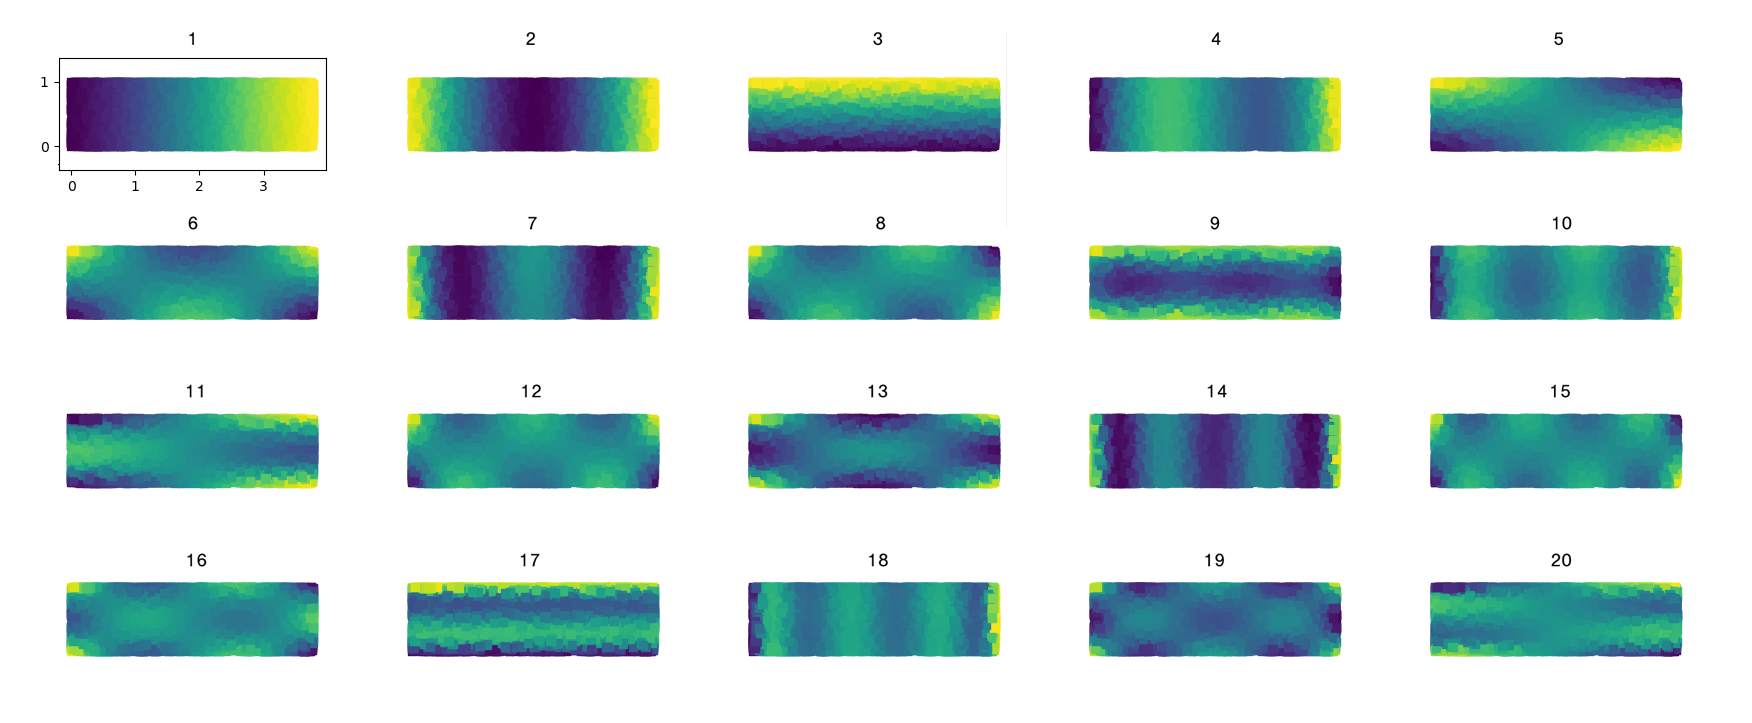
\includegraphics[width=\textwidth]{images/line_line_eigenvalues_20.png}
    \caption{The 20 most significant (lowest frequency) Laplace eigenvectors of data sampled over a rectangle $\Omega = \ell_1 \times \ell_2$. We can easily pick out the base eigenvectors of both underlying lines which form the rectangle, as they distinctively approximate cosines of increasing frequency, which are exactly the Laplace eigenfunctions of the line. The remaining eigenvectors are mixture eigenvectors of base eigenvectors from $\ell_1$ and $\ell_2$. For example, in the top row we can easily see that the eigenvector 5 is a mixture of eigenvector 1 and eigenvector 3.}
    \label{fig:rect_eigenvectors}
\end{figure}

\begin{figure}[ht]
    \centering
    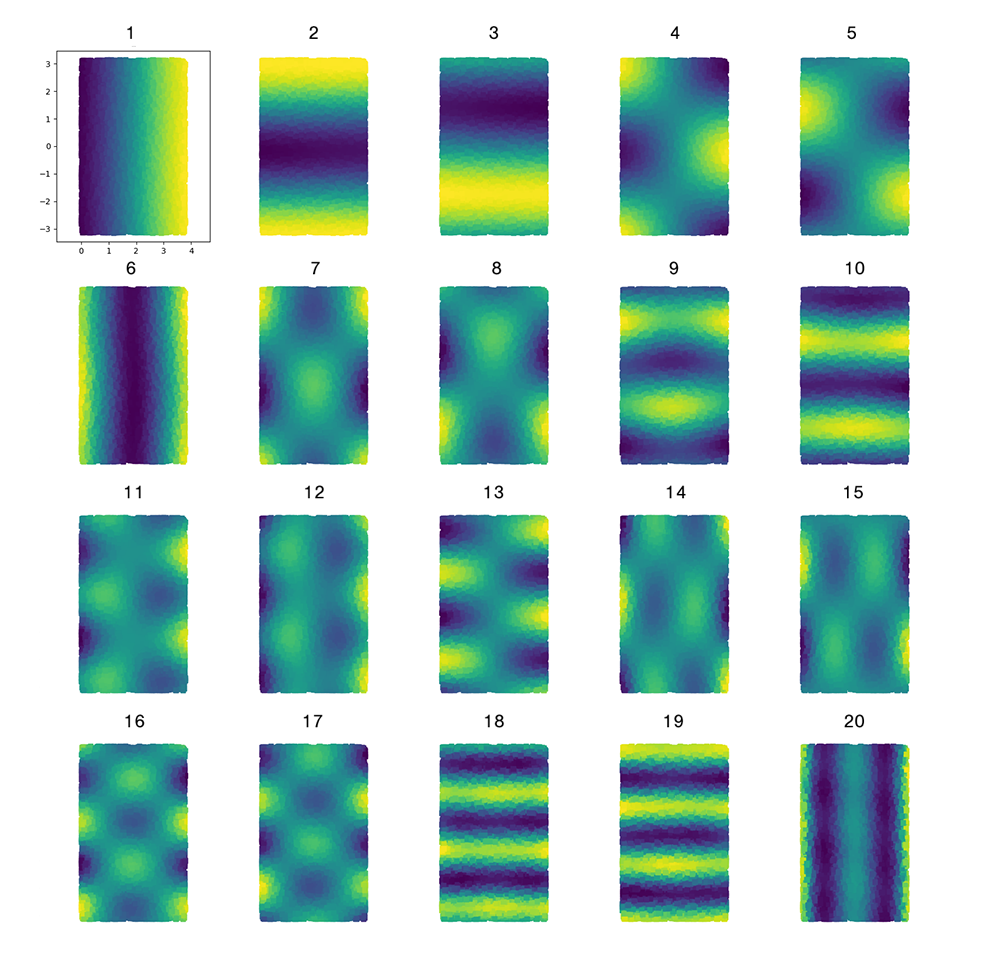
\includegraphics[width=0.8\textwidth]{images/line_circle_eigenvalues_20.png}
    \caption{The 20 most significant eigenvectors of data sampled over a hollow cylinder, which can be represented by $\Omega = \ell \times \theta$. The base eigenvectors of $\ell$ approximate cosine functions from left to right, and the base eigenvectors of $\theta$ approximate sine and cosine functions.}
    \label{fig:cyl_eigenvectors}
\end{figure}

\begin{exmp}[Rectangle]
Consider a rectangle $\Omega = [0, a] \times [0, b]$. The Laplace eigenproblem is
\begin{equation}\label{laplace_eq1}
\Delta u + \lambda u = u_{xx} + u_{yy} + \lambda u = 0, \quad 0 < x < a, \quad 0 < y < b
\end{equation}
with Neumann boundary conditions
\begin{equation}\label{boundary_cond1}
u_x(0,y) = u_x(a,y) = 0, \quad u_y(x,0) = u_y(x,b) = 0.
\end{equation}

We start with separation of variables. Let $u = X(x)Y(y)$, so the Laplace equation becomes
\begin{equation}
    X''Y + Y''X = -\lambda XY
\end{equation}
and so
\begin{equation}
   \frac{X''}{X} = -\frac{Y''}{Y} - \lambda.
\end{equation}
The left hand side only depends on $x$ and the right hand side only depends on $y$, so both must be constant. Moreover, this constant must be negative (we will show this later). Thus
\begin{equation}\label{eq2}
    \frac{X''}{X} = -\alpha^2, \quad \frac{Y''}{Y} = \lambda - \alpha^2 = -\beta^2
\end{equation}
and this gives us
\begin{equation}\label{eq3}
X'' = -\alpha^2 X, \quad Y'' = -\beta^2 Y
\end{equation}
subject to boundary conditions
\begin{equation}
X'(0) = X'(a) = 0, \quad Y'(0) = Y'(b) = 0.
\end{equation}
The familiar solutions are $X = \cos(kx)$, $Y = \cos(\ell y)$. Furthermore, our boundary conditions require that $ka = m\pi$ and $\ell b = n\pi$ for $m,n = 0, 1, 2, \ldots$ so we have $k = \frac{m\pi}{a}$ and $\ell = \frac{n\pi}{b}$ for integers $m,n$. Therefore our separated solutions are
\begin{equation}
X_m(x) = A\cos\bigg(\frac{m\pi}{a}x\bigg), \quad Y_n(y) = B\cos\bigg(\frac{n\pi}{b}y\bigg)
\end{equation}
with eigenvalues
\begin{equation}
\lambda_m = \frac{m^2\pi^2}{a^2}, \quad \lambda_n = \frac{n^2\pi^2}{b^2},
\end{equation}
respectively. Combining these solutions gives us our final solutions
\begin{equation}\label{eq4}
u_{m,n}(x,y) = A_{m,n}\cos\bigg(\frac{m\pi}{a}x\bigg)\cos\bigg(\frac{n\pi}{b}y\bigg)
\end{equation}
with eigenvalues
\begin{equation}\label{eq5}
\lambda_{m,n} = \lambda_m + \lambda_n = \pi^2\bigg(\frac{m^2}{a^2} + \frac{n^2}{b^2}\bigg)
\end{equation}
for all possible combinations of nonnegative integers $m$ and $n$. In particular, these are precisely the combinations of eigenfunctions sampled over two independent lines of length $a$ and $b$.

In Figure \ref{fig:rect_eigenvectors}, we show the first $20$ nontrivial eigenvectors calculated from $10,000$ uniform random samples over the rectangle $[0,1] \times [0, \sqrt{\pi}+2]$. As discussed before, these eigenvectors are discrete approximations of the eigenfunctions computed above.
\end{exmp}

\begin{exmp}[Hollow cylinder]
The Laplace eigenproblem for a hollow cylinder is similar to that of the rectangle, but we have slightly different boundary conditions. The problem is stated as
\begin{equation}\label{laplace_eq2}
\Delta u + \lambda u = u_{xx} + u_{\theta\theta} + \lambda u = 0, \quad 0 < x < a, \quad 0 < \theta < 2\pi
\end{equation}
with Neumann boundary conditions
\begin{equation}\label{boundary_cond2}
u_x(0,\theta) = u_x(a,\theta) = 0.
\end{equation}

Again, we first use separation of variables to write $u(x,\theta) = X(x)\Theta(\theta)$. The solution for $X$ is identical to the example over a rectangle, and the solutions for $\Theta$ are the same as those in Examples \ref{laplace-disk}. This gives us
\begin{equation}
X_m(x) = \cos\Big(\frac{m\pi}{\ell}x\Big), \quad \Theta_n(\theta) = A_n\cos(n\theta) + B_n\sin(n\theta)
\end{equation}
with eigenvalues
\begin{equation}
\lambda_m = \frac{m^2\pi^2}{\ell^2}, \quad \lambda_n = n^2,
\end{equation}
respectively. The Laplace eigenfunctions of the hollow cylinder are then
\begin{equation}
u_{m,n}(x, \theta) = A_n\cos\Big(\frac{m\pi}{\ell}x\Big)\cos(n\theta) + B_n\cos\Big(\frac{m\pi}{\ell}x\Big)\sin(n\theta)
\end{equation}
with eigenvalues
\begin{equation}
\lambda_{m,n} = \lambda_m + \lambda_n = \frac{m^2\pi^2}{\ell^2} + n^2.
\end{equation}
Figure \ref{fig:cyl_eigenvectors} shows the first 20 nontrivial eigenvectors calculated from $10,000$ uniform random samples over the hollow cylinder of radius $r$ and height $\ell$.
\end{exmp}

\subsection{Graph Laplacians and diffusion maps}
The results of the previous sections hold for the continuous Laplacian, but in practice we may be unable to simulate the continuous case. In this section, we introduce the graph Laplacian, which is a discrete version of the continuous Laplacian. While data is inherently discrete, the authors of \cite{Nadler_2006} show that for large sample sizes the discrete analogs of the spectrum of the Laplacian provide good approximations of the actual spectrum. We also show the relationship between the graph Laplacian and diffusion maps, which are an important component of our algorithm. For further exposition, refer to \cite{coifman2006diffusion} and \cite{Belkin_2003}.

The discrete Laplacian is defined over a graph $(G,E,V)$, which we can interpret as a representation of $\mathbf{x}_1, \ldots \mathbf{x}_n \in \mathbb{R}^D$. In order to capture the relationships within our data, we define a weight matrix $W$ where
\begin{equation}
W_{ij} = k\bigg(\frac{||x_i-x_j||^2}{2\sigma}\bigg),
\end{equation}
with $k$ being the Gaussian kernel. We can then define the random walk matrix $A = D^{-1}W$, where $D$ is the diagonal degree matrix defined by
\begin{equation}\label{degree_matrix}
D_{ii} = \sum_{j=1}^m W_{ij}.
\end{equation}
The matrix $A$ describes the probability cloud of a random walk on $G$, which can be used as a model for the connectivity between points in the data. The idea is that a random walker on this graph is always more likely to move from its current position to another point that is strongly similar, rather than another point that is less similar. Hence, after a long time, the distribution of the random walk describes the underlying geometry of the data. A lower-dimensional embedding of the data using the diffusion map essentially reorganizes the data so that the Euclidean distance between data points in the lower-dimensional space approximates their connectivity in the kernel space.

The diffusion map is a mapping from each point $i \mapsto A^t[i,:]$, which describes the distribution of a random walker's location at time $t$, given that the initial location was at point $v_i$. To compute $A$, we instead consider the symmetric matrix
\begin{equation}\label{def:S}
    S = D^{\frac{1}{2}}AD^{-\frac{1}{2}} = D^{-\frac{1}{2}}WD^{-\frac{1}{2}},
\end{equation}
as $A$ is not symmetric. We then take the eigendecomposition
\begin{equation}
    S = V\Sigma V^T
\end{equation}
and substitute it back into (\ref{def:S}) to obtain
\begin{equation}
A = D^{-\frac{1}{2}}SD^{\frac{1}{2}} = D^{-\frac{1}{2}}V\Sigma V^TD^{\frac{1}{2}} = \big(D^{-\frac{1}{2}}V\big)\Sigma\big(D^{\frac{1}{2}}V\big)^T.
\end{equation}
Define $\Phi = D^{-\frac{1}{2}}V = [\varphi_1, \ldots, \varphi_d]$ and $\Psi = D^{\frac{1}{2}}V = [\psi_1, \ldots, \psi_d]$, where $\phi_i, \psi_i \in \mathbb{R}^n$. This gives us the decomposition
\begin{equation}
A = \Phi \Sigma \Psi^T.
\end{equation}
Now, $A\varphi_i = \lambda_i\varphi_i$ and $\psi^T_iA = \lambda\psi^T_i$, i.e., $\phi_i$ and $\psi_i$ are the right and left eigenvectors of $A$. Moreover, $\psi^T_j \varphi_j = 1$, so we can write

\begin{equation}
    M = \sum_{j=1}^n \lambda_j \varphi_j \psi^T_j, \quad M^t = \sum_{j=1}^n \lambda^t_j \varphi_j \psi^T_j.
\end{equation}
Then our mapping can be written as
\begin{equation}
    i \mapsto M^t[i,:] = \sum_{j=1}^n \lambda^t_j \varphi_j(i)\psi^T_j
\end{equation}
and so each point can be represented entirely by the basis $\{\psi_j\}_{j=1}^d$ and its coefficients $(\lambda^t_1\varphi_1(i) \cdots \lambda^t_n\varphi(n))$. 

Observe that $A\mathbf{1} = \mathbf{1}$ by virtue of its probabilistic construction, so one of the eigenvalues will always be $1$. Moreover, it can be shown that $|\lambda_j| \le 1$ for all $j$. Thus $\lambda_1$ and $\varphi_1$ are uninteresting, and we can define a truncated diffusion map
\begin{equation}
    i \mapsto (\lambda^t_1\varphi_1(i), \cdots ,\lambda^t_{d+1}\varphi(d+1)).
\end{equation}

The graph Laplacian is given by $L = I - A$, where $I$ is the $n \times n$ identity matrix. The largest eigenvalues and corresponding eigenvectors of $L$ can be computed for further spectral analysis methods such as spectral clustering and dimensionality reduction. It can be easily seen that the eigenvectors of $L = I-A$ are precisely the eigenvectors of $A$. Therefore, calculating $\Phi$ will give us the $d$ most significant Laplace eigenvectors of $L$.

\subsection{Limit of the graph Laplacian}
Ideally, we would like our Laplace eigenvectors to act as discrete approximations of the actual Laplace eigenfunctions of the data manifold. Fortunately, this is the case for a sufficiently large sample of data. If the data $\{\mathbf{x}_i\}_{i=1}^n$ is uniformly distributed over $\mathcal{M}$, Belkin and Niyogi show in \cite{Belkin_2008} that the graph Laplacian converges to the continuous Laplace operator $\Delta_M$ over $\mathcal{M}$. If the data instead has a general distribution $p(x)$, the graph Laplacian converges to the backward Fokker-Planck operator, 
\begin{equation}\label{fokker-placnk}
    \mathcal{L}f = \Delta_M f - \nabla U \cdot \nabla f
\end{equation}
where $U(x) = -2\log p(x)$ is a potential function \cite{Nadler_2006}. Moreover, the eigenvectors of $L$ are discrete approximations of the eigenfunctions of the continuous Laplacian with homogeneous Neumann boundary conditions,
\begin{align}
    &\Delta_M f(x) = \lambda f(x), \quad x \in \mathcal{M} \\
    &\frac{\partial f}{\partial \nu} = 0, \quad x \in \partial \mathcal{M}
\end{align}
where $\nu$ is the normal vector to the boundary $\partial\mathcal{M}$ at $x$.

While the results above assume a submanifold of $\mathbb{R}^D$, this discussion can be extended to general manifolds as well \cite{Belkin_2008}. For the purposes of our exploration, we will not consider these generalizations. In the remainder of this paper, we restrict our experiments to submanifolds $\mathcal{M} \mathbb{R}^D$ which are the product of two independent domains $\mathcal{M}_1$ and $\mathcal{M}_2$. Thus every eigenfunction of $\mathcal{M}$ can be written as $f_j g_k$ with eigenvalue $\lambda_j + \mu_k$, where $f_j$ is a Laplace eigenfunction of $\lambda_j$ over $\mathcal{M}_1$ and $g_k$ is a Laplace eigenfunction of $\mu_k$ over  $\mathcal{M}_2$.

\section{Method}
\subsection{Predicting base eigenvectors}
As we have shown, any Laplace eigenvector $\varphi_k$ for data sampled from the product manifold $\mathcal{M} = \mathcal{M}_1 \times \mathcal{M}_2$ can be written as the element-wise product
\begin{equation}
\varphi^{(i,j)} = \varphi^{(1)}_i \varphi^{(2)}_j,
\end{equation}
where $\varphi^{(1)}_i$ is an eigenvector of $\mathcal{M}_1$ and $\varphi^{(2)}_j$ is an eigenvector of $\mathcal{M}_2$. If $\varphi^{(b)}_k$ is the trivial eigenvector $\mathbf{1}$ for $b = 1,2$, we call $\varphi^{(i,j)}$ a \textit{base} eigenvector of $\mathcal{M}_{3-b}$, otherwise we say it is a \textit{mixture} eigenvector. We now present a method for determining the base eigenvectors included in the first $N$ Laplace eigenvectors of $\mathcal{M}$.

We begin by finding all triplets of eigenvectors $(\varphi_i, \varphi_j, \varphi_k)$ such that $\varphi_k$ best matches the element-wise product of $\varphi_i$ and $\varphi_j$. To do so, we iterate through all triplets $(\varphi_i, \varphi_j, \varphi_k)$ where $i < j < k \le N$, and check how ``close" $\varphi_i\varphi_j$ is to $\varphi_k$. Here, ``closeness" is measured by scaling $\varphi_i\varphi_j$ and $\varphi_k$ exactly into the range $[-1, 1]$ and computing the L1-norm of the difference between the two scaled vectors. We make sure to check both $\varphi_k$ and $-\varphi_k$, as the sign of the first two eigenvectors relative to the third eigenvector is not known. The $\varphi_k$ that is closest to $\varphi_i\varphi_j$ is recorded, as well as the distance. Finally, since we only want to work with reliable triplets, we filter out all of the resulting $\genfrac(){0pt}{2}{N}{2}$ triplets which have a distance above a certain threshold. The algorithm is summarized in Algorithm \ref{alg1} below. \\

\begin{algorithm}[H]\label{alg1}
\SetAlgoLined
\KwResult{Constructs a list of eigenvector triplets $(\varphi_i, \varphi_j, \varphi_k)$}
\code{bestTriplets} $\gets Array()$\;
 \For{$i\gets1$ \KwTo $N-2$}{
    \For{$j\gets i+1$ \KwTo $N-1$}{
        \code{product} $\gets normalize(\varphi_i\varphi_j)$\;
        \code{closestDist} $\gets 0$, \code{closest} $\gets None$\;
        \For{$k\gets j+1$ \KwTo $N$}{
            \code{candidateDist} $\gets |\pm\varphi_k - \code{product}|$\;
            \If{\code{candidateDist} $<$ \code{closestDist}}{
                \code{closestDist} $\gets$ \code{candidateDist}, \code{closest} $\leftarrow \varphi_k$\;
            }
        }
        \If{\code{closestDist} $< d$}{
            add $(\varphi_i, \varphi_j, \varphi_k)$ to \code{bestTriplets}\;
        }
    }
 }
 return \code{bestTriplets}\;
 \caption{Searching for reliable triplets}
\end{algorithm}
\vspace{0.25cm}
The result of the algorithm is a list of triplets indicating which eigenvectors are likely to be base eigenvectors (the first two eigenvectors in each triplet), and which eigenvectors are likely to be mixture eigenvectors (the third eigenvector in each triplet).

\subsection{Separating base eigenvectors}
Let $\mathcal{T}$ be our list of triplets. We will use a voting procedure to determine which manifold each eigenvector is associated with. Since it is not guaranteed that there exists a division or a unique division that is characterized by our list of triplets, we opt for a spectral approach. First, define $T = \{\varphi_1, \ldots, \varphi_t\}$ to be the set of eigenvectors found in our list of triplets. We will construct a complete weighted graph $(G,E,V)$ where each vertex corresponds to an eigenvector in $T$, and each edge has a weight $w_{ij}$ representing the affinity between $\varphi_i$ and $\varphi_j$. A higher affinity indicates that the two eigenvectors likely belong to the same intrinsic manifold. 

We will also keep track of the number of times an eigenvector appears as a base eigenvector or a mixture eigenvector in each triplet via a voting system. For every time that an eigenvector appears as a base eigenvector we cast it one vote, and every time that an eigenvector appears as a mixture eigenvector we subtract one vote for it. Let $v(i)$ denote the net number of votes that eigenvector $\varphi_i$ receieves. We include in our affinity matrix only edges between eigenvectors which have receieved more than $K$ net votes. To construct the votes and weights for $G$, we iterate through each triplet $(\varphi_i, \varphi_j, \varphi_k)$ in $\mathcal{T}$ and collect votes for edges and vertices as follows:
\begin{itemize}
    \item Add 1 to each of $w_{ij}$ and $w_{ji}$
    \item Add 1 to each of $v(i)$ and $v(j)$
    \item Subtract 1 from $v(k)$
\end{itemize}
After going through all triplets in $\mathcal{T}$, the edges between eigenvectors which appeared most frequently together as well-paired base eigenvectors will have large distances between them, and eigenvectors which appeared most as base eigenvectors have the highest votes. Applying a Gaussian kernel to these distances produces an affinity matrix which can then be used for spectral clustering \cite{von_Luxburg_2007, scikit-learn}. The final algorithm is summarized in Algorithm \ref{alg2}. \\

\begin{algorithm}[H]\label{alg2}
\SetAlgoLined
\KwResult{Given a list $\mathcal{T}$ of triplets and $K$, computes two lists of base eigenvectors associated with $\mathcal{M}_1$ and $\mathcal{M}_2$}
 initialize $W \gets Array(t,t)$\;
 \For{$(\varphi_i,\varphi_j,\varphi_k)$ in $\mathcal{T}$}{
    $W(i,j) \gets W(i,j) + 1$\;
    $W(j,i) \gets W(j,i) + 1$\;
    $v(i) \gets v(i) + 1$, $v(j) \gets v(j) + 1$, $v(k) \gets v(k) - 1$\;
 }
 Restrict $W$ to the eigenvectors $\{\varphi_i : v(i) \ge K\}$\;
 $W \gets \exp(-W)$ elementwise\;
 $\code{eigenvectors1}, \code{eigenvectors2} \gets$ \code{SpectralClustering}($W$, \textit{clusters}$=2$)\;
 return \code{eigenvectors1}, \code{eigenvectors2}\;
 \caption{Spectral procedure to separate base eigenvectors}
\end{algorithm}

\begin{rem}
The case of $m=2$ clusters in Algorithm 2 can be done without spectral clustering. Instead, we can compute the \textit{Fiedler vector}, which is the eigenvector of the graph Laplacian with the smallest positive eigenvalue and separate the vertices based on the entries in this eigenvector. Vertices corresponding to positive entries of the eigenvector belong to one cluster, and all the other vertices belong to the other cluster.
\end{rem}

\section{Results}
To test the algorithm, we ran it on two two-dimensional toy manifolds, a rectangle and a hollow cylinder. The ground truth Laplace eigenfunctions of both manifolds are known, as derived in Section 2. For each manifold, we collect 10,000 uniform random samples over the ambient manifold, and we examine the 100-dimensional diffusion map created from those samples, which give us the first 100 nontrivial Laplace eigenvectors. The default parameters are set to $d=0.08, K=2$ for the rectangle and $d=0.12, K=2$ for the hollow cylinder, but we also explore the effects of varying these parameters.

\begin{figure} 
    \centering
    \begin{subfigure}[t]{\textwidth}
        \centering
        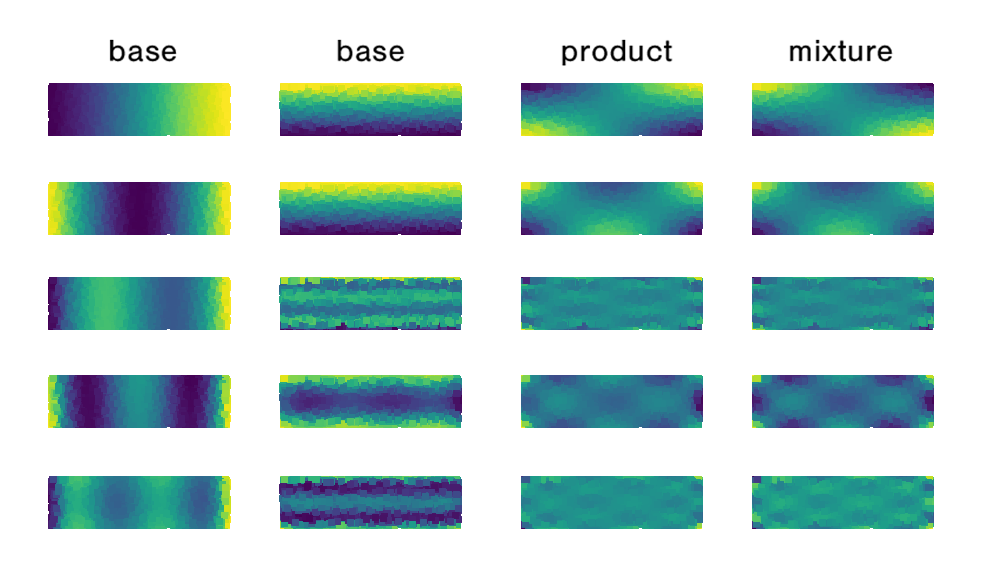
\includegraphics[width=\textwidth]{images/line_line_matches.png}
        \caption{Rectangle}
    \end{subfigure}
    \begin{subfigure}[t]{\textwidth}
        \centering
        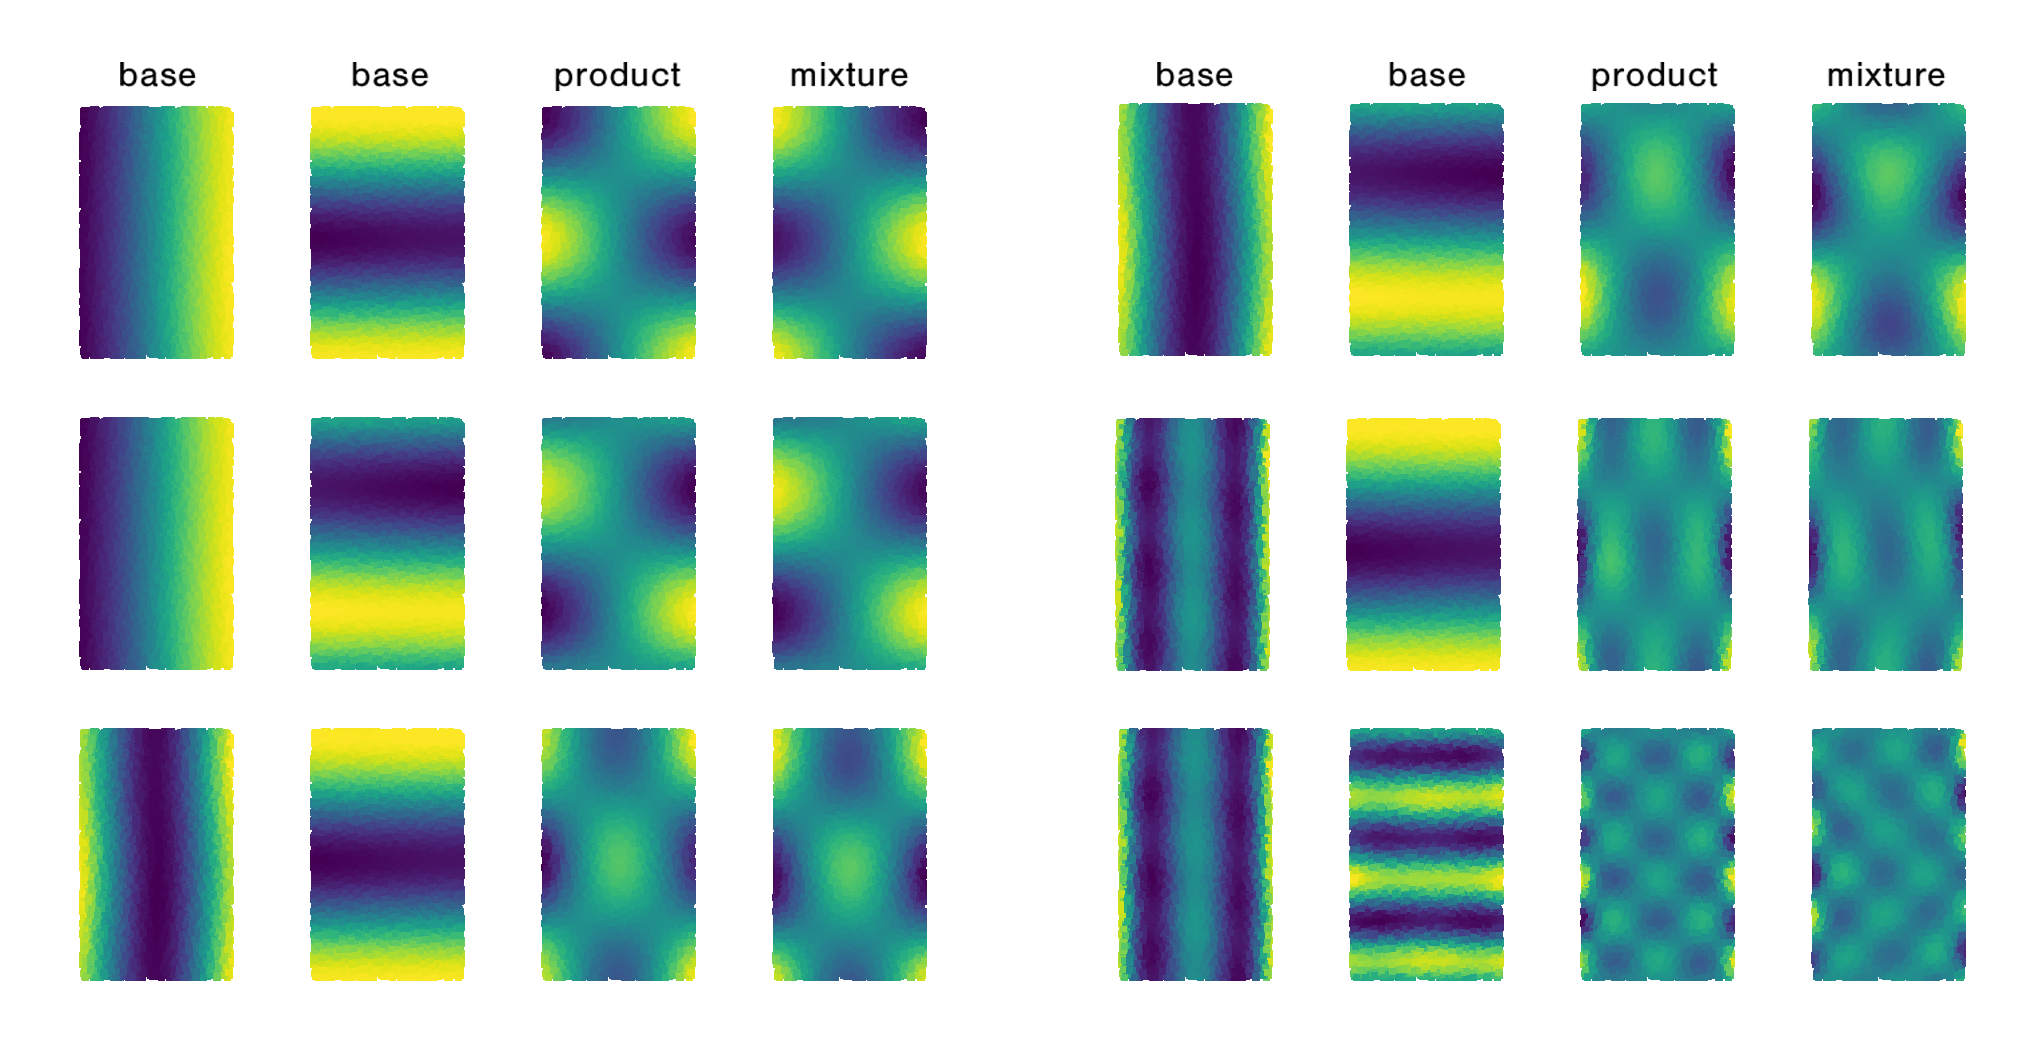
\includegraphics[width=\textwidth]{images/line_circle_matches.png}
        \caption{Hollow cylinder}
    \end{subfigure}
    \caption{Some of the mixture eigenvectors compared to products of base eigenvectors chosen by the algorithm. The two columns on the left show base vectors from separate manifolds determined by the algorithm. The \textit{product} column shows the elementwise product of the two left columns, and the \textit{mixture} column shows the closest actual mixture eigenvector found by the algorithm. The alignment between the last two columns indicates that the Euclidean L1-distance is an effective way of determining mixture eigenvectors.}
    \label{fig:combos}
\end{figure}

The results are shown in Figures \ref{fig:rectangle} and \ref{fig:cylinder}. The algorithm produces two groups of base eigenvectors, each corresponding to an independent manifold. In both of these examples, the algorithm is able to accurately determine the most significant base eigenvectors associated with each independent submanifold, as well as some higher frequency eigenvectors. Comparisons between the results and the ground truth eigenvectors show that the algorithm consistently identifies several of the lowest frequency eigenfunctions. Note that some eigenvectors in Figures \ref{fig:rectangle} and \ref{fig:cylinder} are mirror images of those in Figure \ref{fig:rect_eigenvectors} and \ref{fig:cyl_eigenvectors}, as the algorithm takes into account both positive and negative scalar multiples of eigenvectors.

In Figure \ref{fig:combos}, we compare the mixture eigenvectors selected by the algorithm compared against the product of the base eigenvectors selected by the algorithm. The product and mixture eigenvectors match extremely closely in structure, up to a sign flip. This indicates not only an accurate separation and choice of base eigenvectors, but also that the L1-distance scoring to determine triplets in Algorithm 1 is effective.

\begin{figure}
    \centering
    \begin{subfigure}[t]{\textwidth}
        \centering
        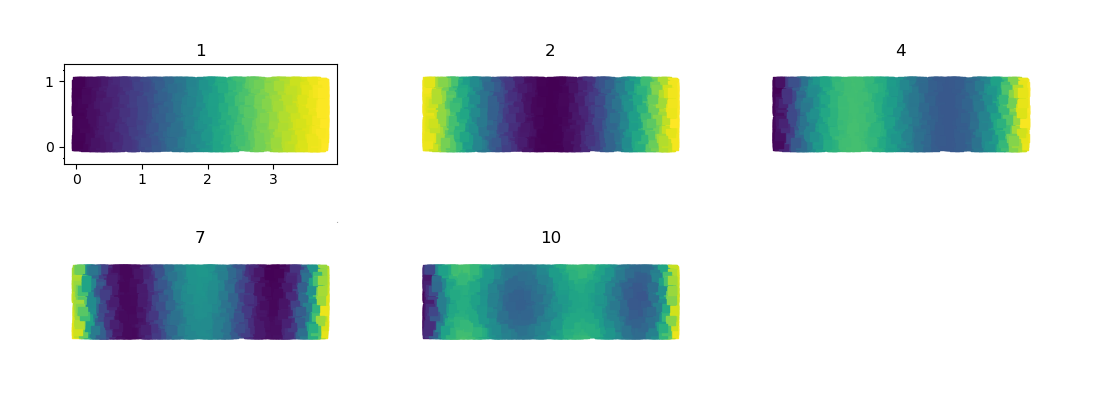
\includegraphics[width=0.49\textwidth]{images/manifold1_line_line2.png}
        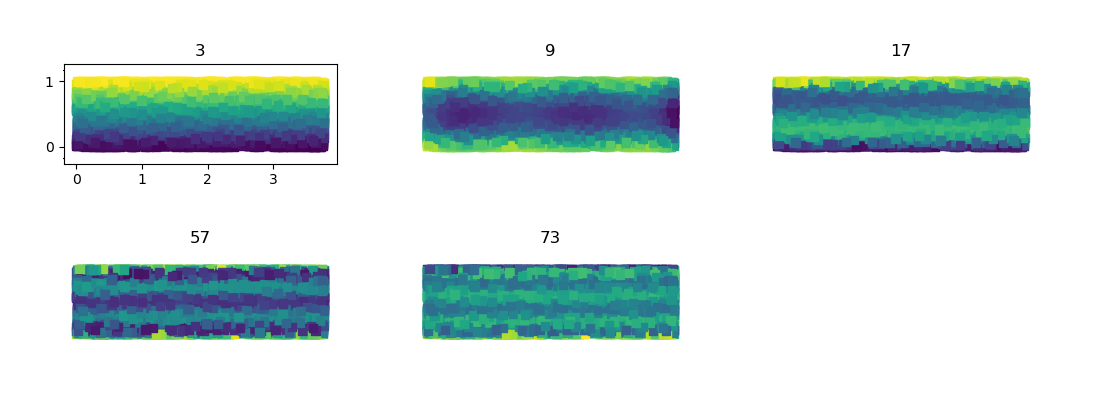
\includegraphics[width=0.49\textwidth]{images/manifold2_line_line2.png}
        \caption{$d=0.08$, $K=2$}
    \end{subfigure}
    \begin{subfigure}[t]{\textwidth}
        \centering
        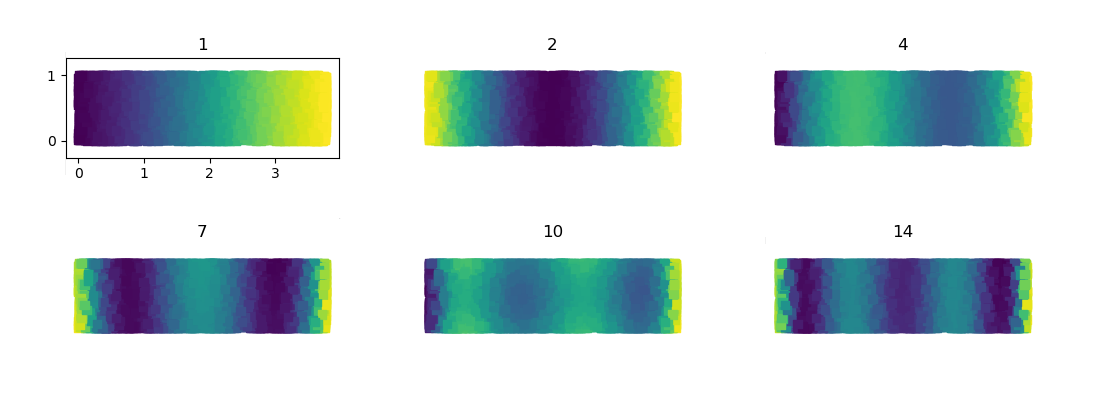
\includegraphics[width=0.49\textwidth]{images/manifold1_line_line3.png}
        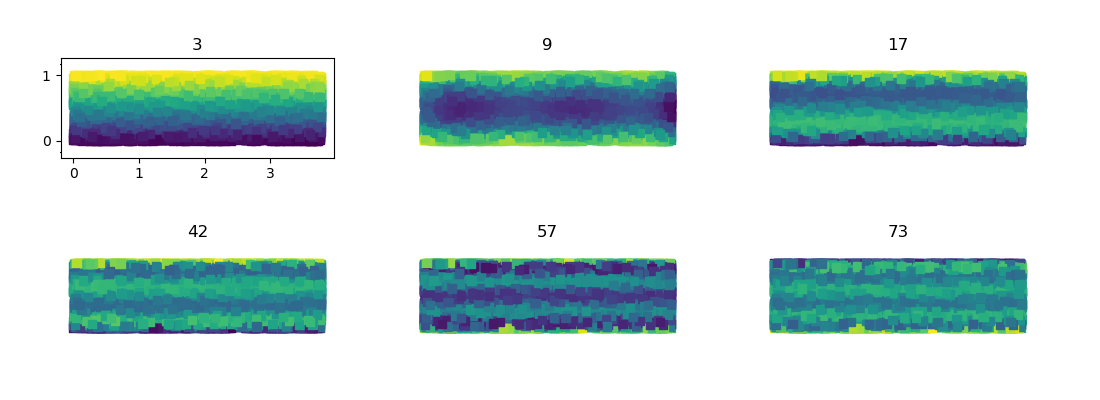
\includegraphics[width=0.49\textwidth]{images/manifold2_line_line3.png}
        \caption{$d=0.25$, $K=3$}
    \end{subfigure}
    \caption{The results of the algorithm on 10,000 points sampled from the rectangle $\Omega = [0, 2 + \sqrt{\pi}] \times [0,1]$. Varying distance and voting thresholds $d$ and $K$ were applied over the same set of samples, resulting in slightly different separations. On the left are the base eigenvectors associated with $l_1 = [0, 2 + \sqrt{\pi}]$, on the right are the base eigenvectors associated with $l_2 = [0,1]$. As we can see, the algorithm is able to consistently pick out the most significant base eigenvectors for both manifolds.}
    \label{fig:rectangle}
\end{figure}

\begin{figure} 
    \centering
    \begin{subfigure}[t]{\textwidth}
        \centering
        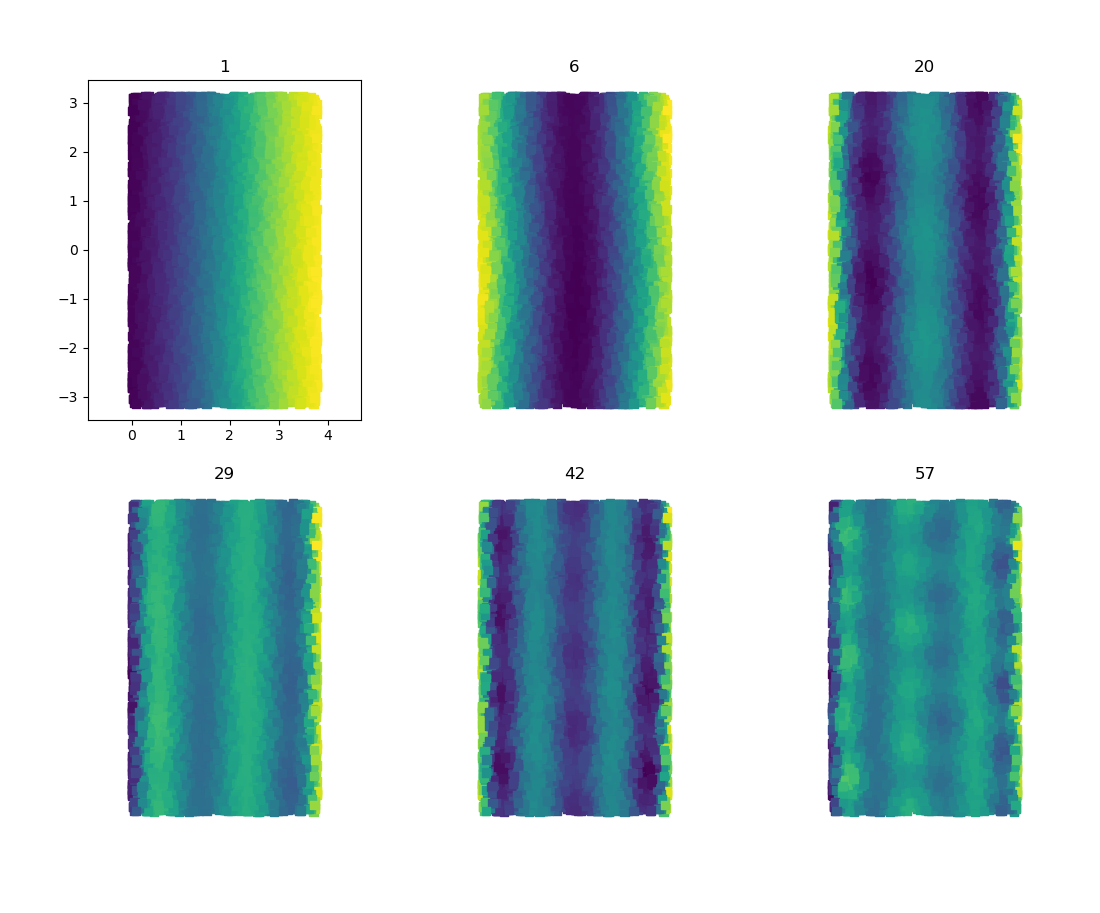
\includegraphics[width=0.42\textwidth]{images/manifold1_line_circle2.png}
        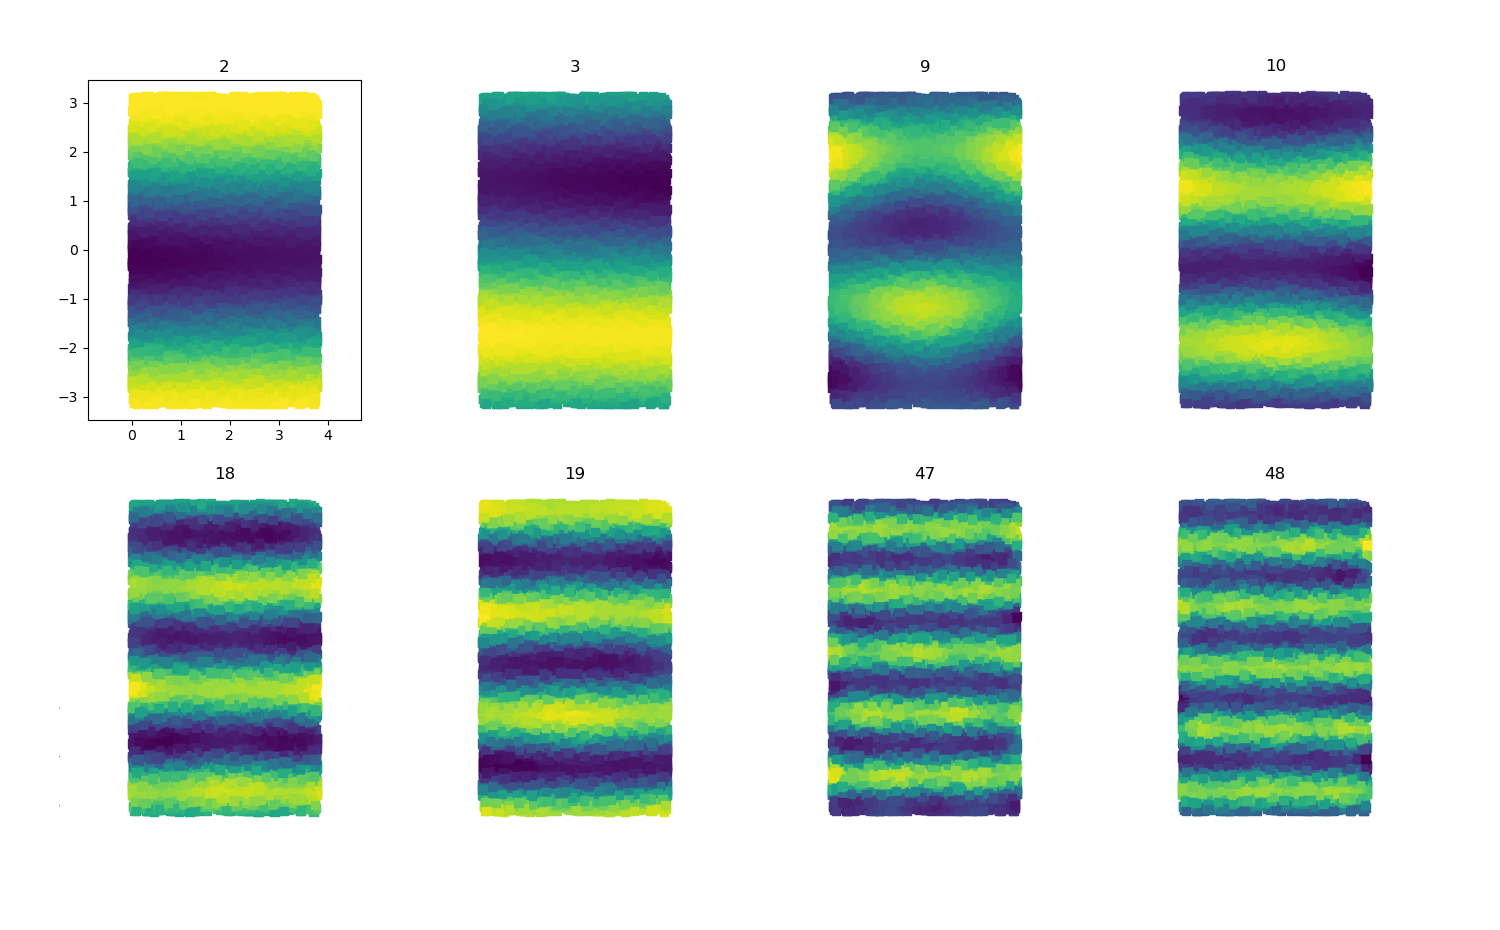
\includegraphics[width=0.56\textwidth]{images/manifold2_line_circle2.png}
        \caption{$d=0.12$, $K=2$}
    \end{subfigure}
    \begin{subfigure}[t]{\textwidth}
        \centering
        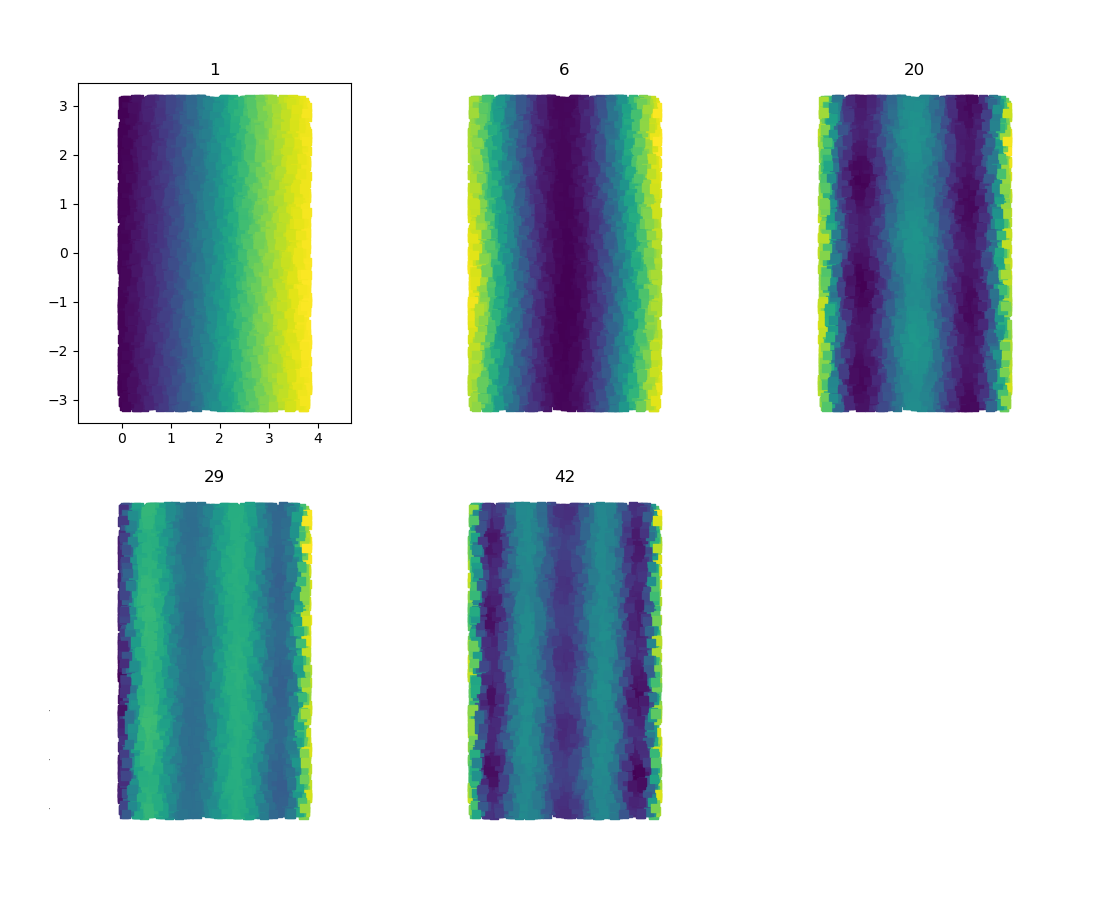
\includegraphics[width=0.42\textwidth]{images/manifold1_line_circle3.png}
        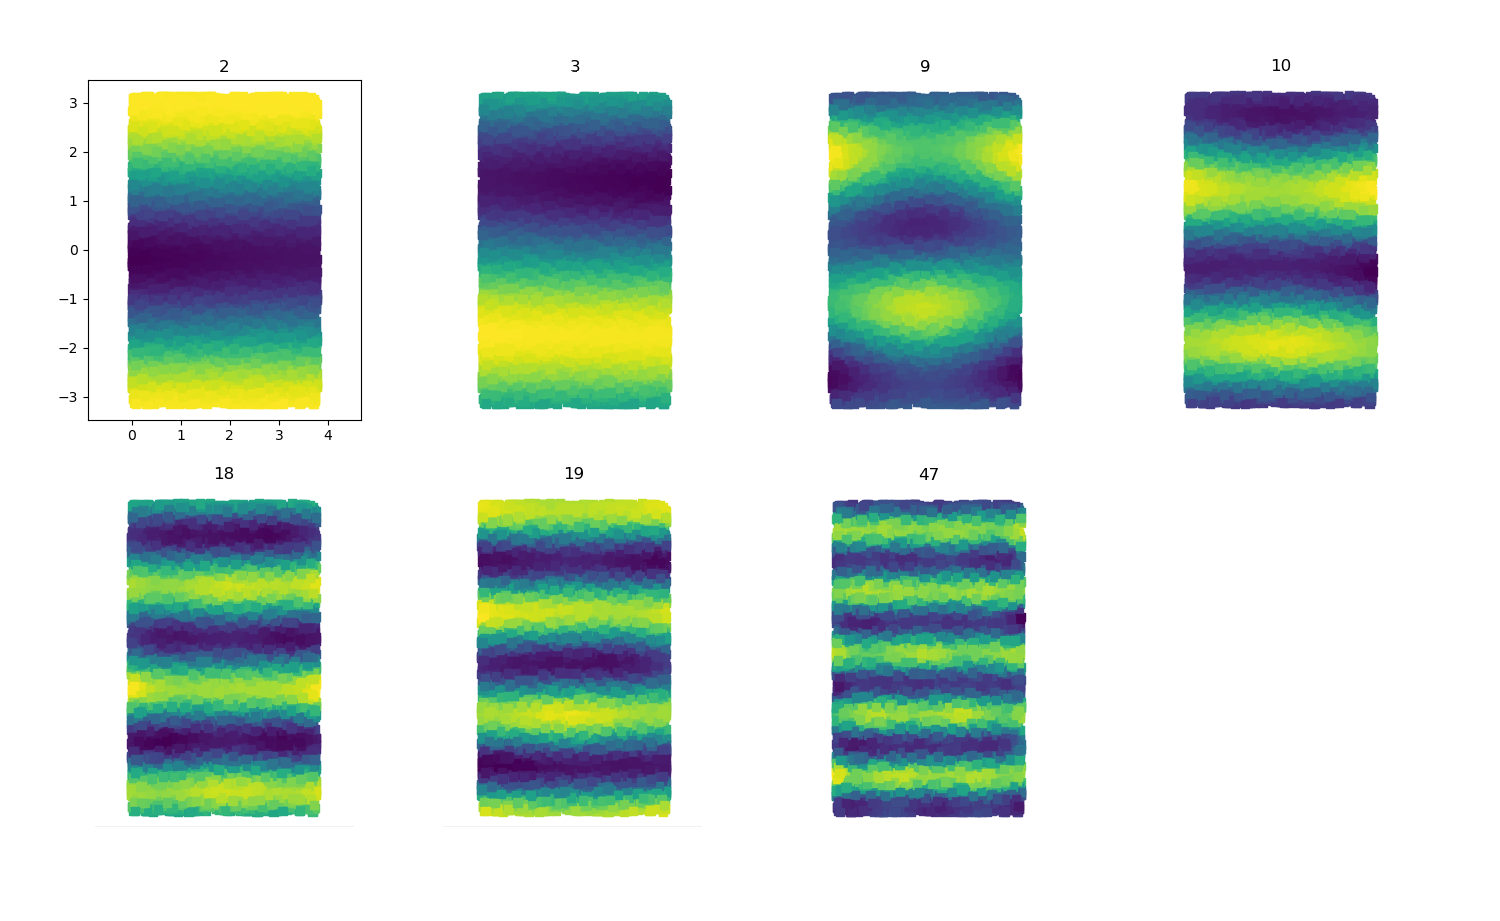
\includegraphics[width=0.56\textwidth]{images/manifold2_line_circle3.png}
        \caption{$d=0.18$, $K=3$}
    \end{subfigure}
    \caption{The results of the algorithm on 10,000 points sampled from the hollow cylinder $\Omega = [0, 2 + \sqrt{\pi}] \times [-\pi, \pi]$. Varying distance and voting thresholds $d$ and $K$ were applied over the same set of samples, resulting in slightly different separations. On the left are the base eigenvectors associated with $l = [0, 2 + \sqrt{\pi}]$, on the right are the base eigenvectors associated with $\theta = [-\pi,\pi]$. Like for the rectangle, the algorithm is able to consistently pick out the most significant base eigenvectors for both manifolds.}
    \label{fig:cylinder}
\end{figure}

The two main parameters of the algorithm are $d$, which is the distance threshold used to filter out unreliable triplets, and $K$, which is the voting cutoff for an eigenvector to be considered in the affinity matrix used for manifold separation. Both parameters serve to limit the amount of information that the clustering portion of the algorithm can access, but act against each other. That is, reducing $d$ filters out more eigenvector triplets (Algorithm 1), so that fewer triplets make it to the voting process. Conversely, lowering $K$ increases the number of eigenvectors in the clustering process (Algorithm 2). Thus, in order to obtain comparable results any large adjustment in one parameter in one direction should be coupled with an adjustment of the other parameter in the same direction. Figures \ref{fig:rectangle} and \ref{fig:cylinder} show how comparable results are as $d$ and $K$ vary simultaneously. Expanding the number of reliable triplets by increasing $d$ and choosing base eigenvectors more selectively by increasing $K$ did not alter the results significantly.

\begin{figure}[ht]
    \centering
    \begin{subfigure}[t]{\textwidth}
        \centering
        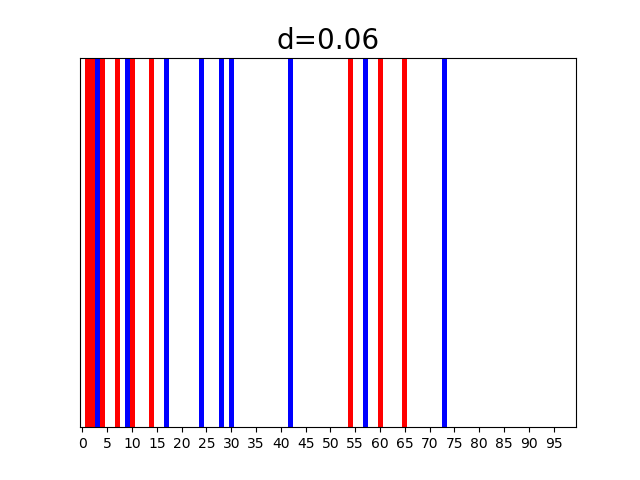
\includegraphics[width=0.2\textwidth]{images/line_line_1_0.06_eigenvector_division.png}
        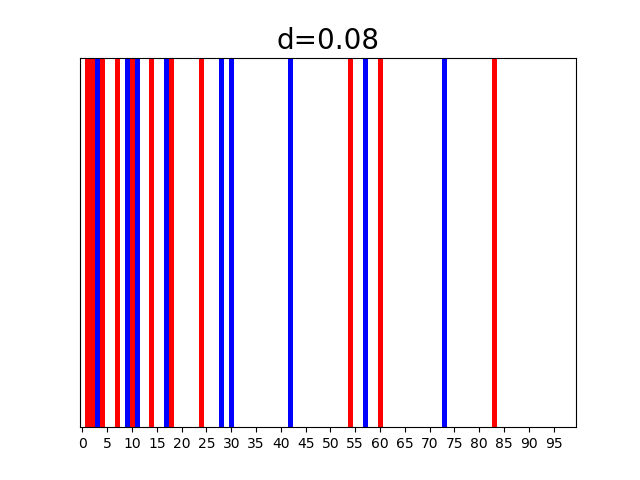
\includegraphics[width=0.2\textwidth]{images/line_line_1_0.08_eigenvector_division.png}
        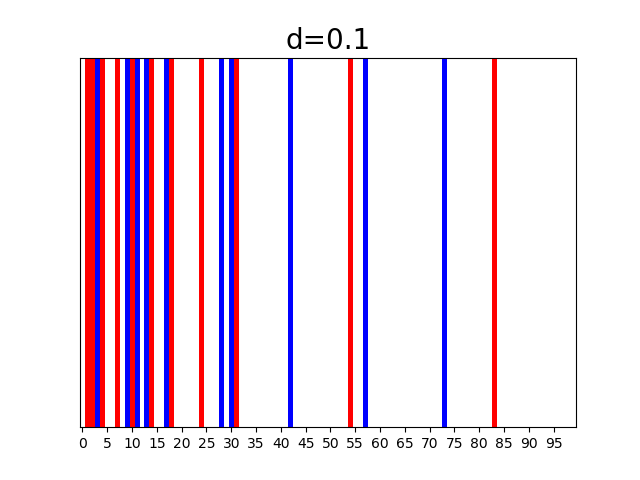
\includegraphics[width=0.2\textwidth]{images/line_line_1_0.1_eigenvector_division.png}
        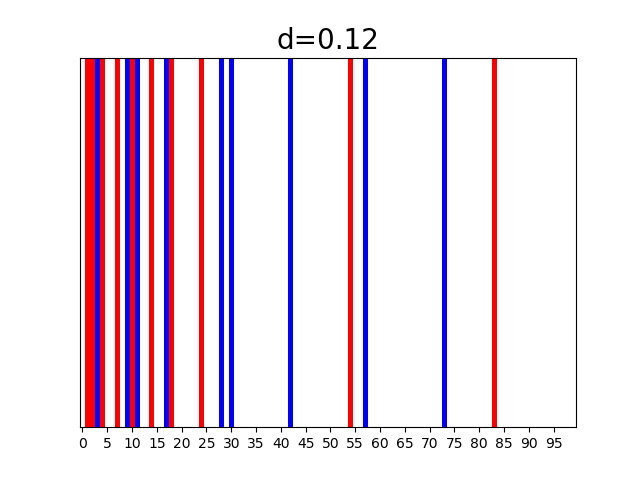
\includegraphics[width=0.2\textwidth]{images/line_line_1_0.12_eigenvector_division.png}
        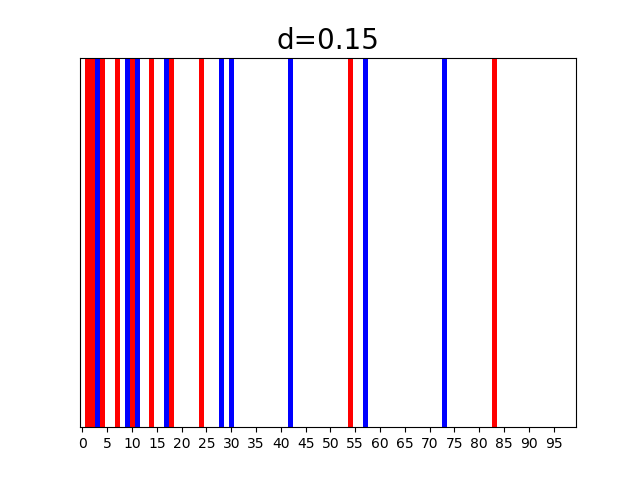
\includegraphics[width=0.2\textwidth]{images/line_line_1_0.15_eigenvector_division.png}
        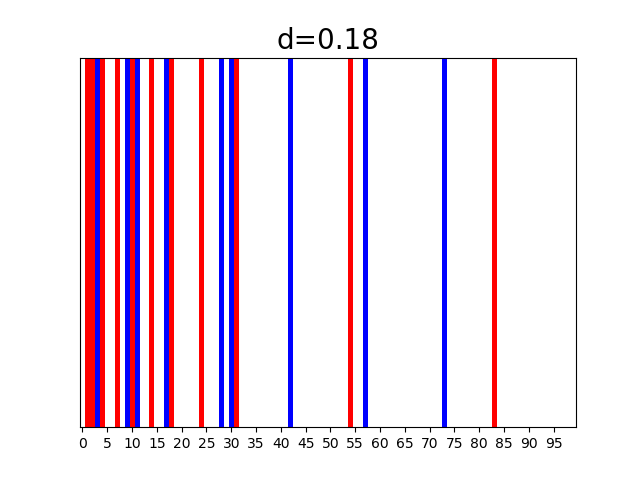
\includegraphics[width=0.2\textwidth]{images/line_line_1_0.18_eigenvector_division.png}
        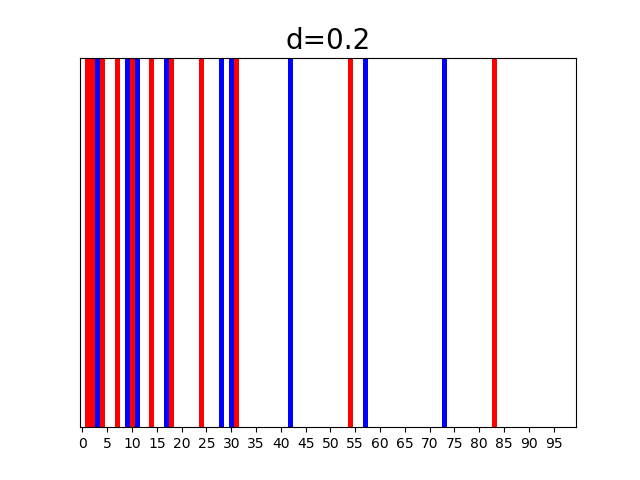
\includegraphics[width=0.2\textwidth]{images/line_line_1_0.2_eigenvector_division.png}
        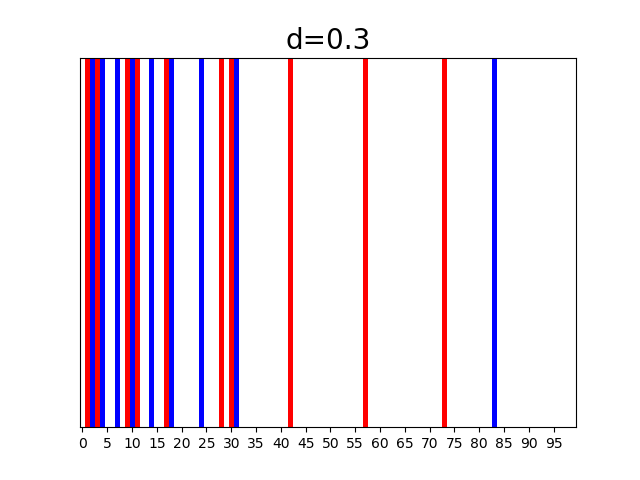
\includegraphics[width=0.2\textwidth]{images/line_line_1_0.3_eigenvector_division.png}
        \caption{Rectangle, $K=1$}
    \end{subfigure}
    \begin{subfigure}[t]{\textwidth}
        \centering
        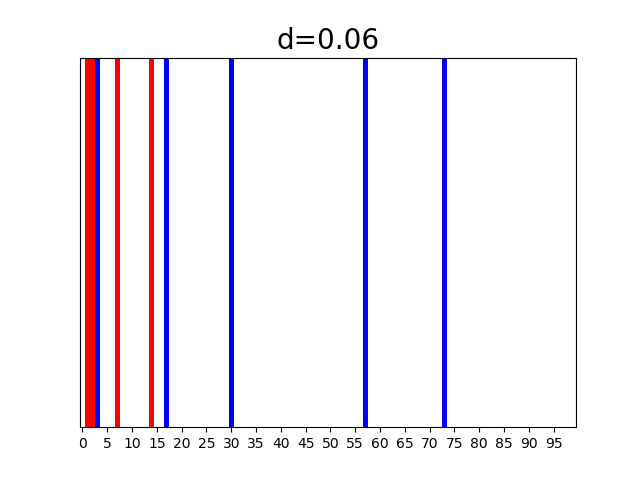
\includegraphics[width=0.2\textwidth]{images/line_line_2_0.06_eigenvector_division.png}
        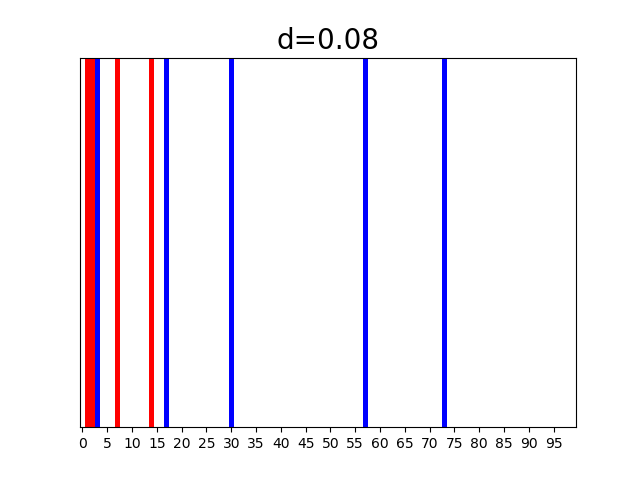
\includegraphics[width=0.2\textwidth]{images/line_line_2_0.08_eigenvector_division.png}
        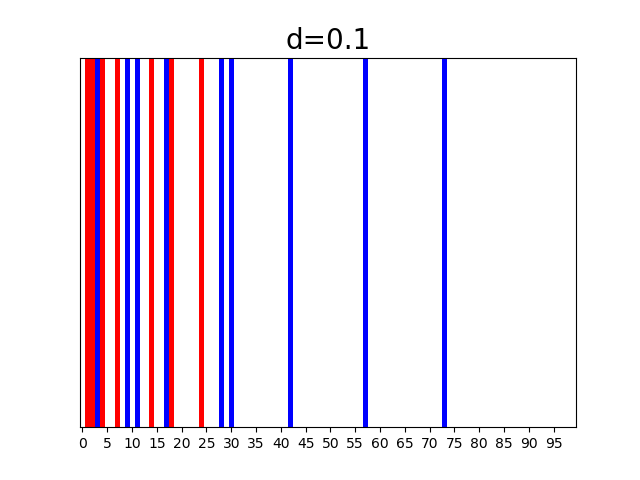
\includegraphics[width=0.2\textwidth]{images/line_line_2_0.1_eigenvector_division.png}
        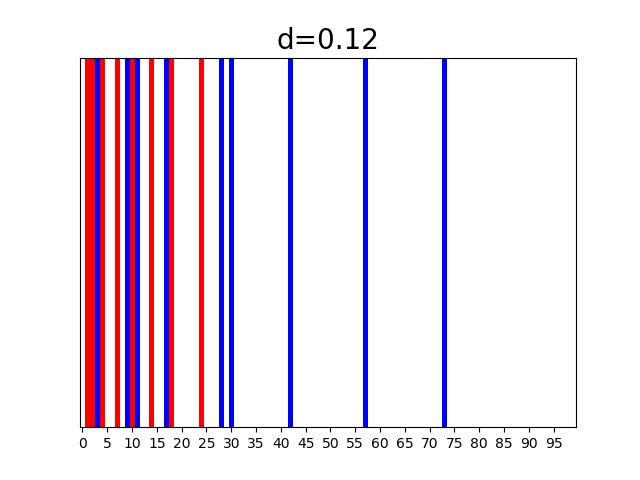
\includegraphics[width=0.2\textwidth]{images/line_line_2_0.12_eigenvector_division.png}
        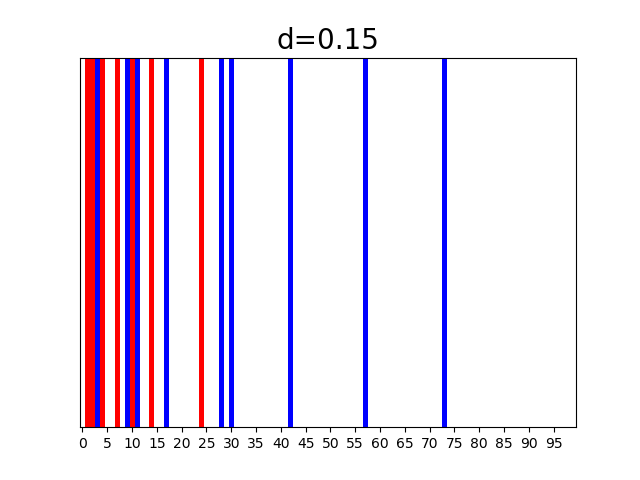
\includegraphics[width=0.2\textwidth]{images/line_line_2_0.15_eigenvector_division.png}
        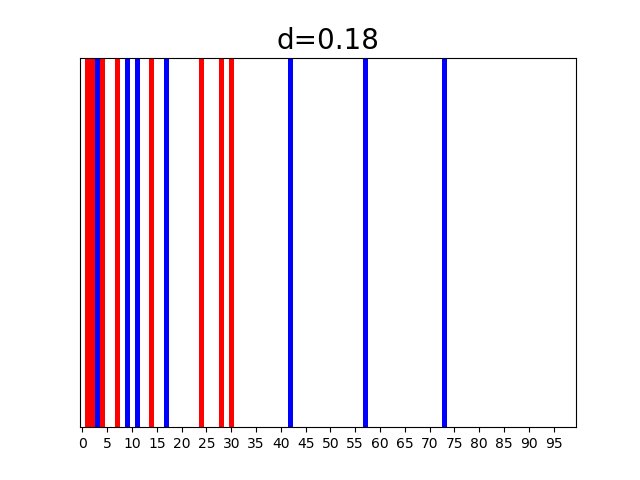
\includegraphics[width=0.2\textwidth]{images/line_line_2_0.18_eigenvector_division.png}
        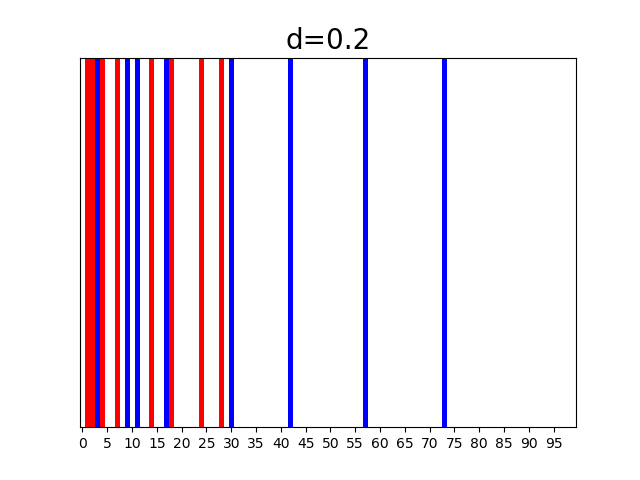
\includegraphics[width=0.2\textwidth]{images/line_line_2_0.2_eigenvector_division.png}
        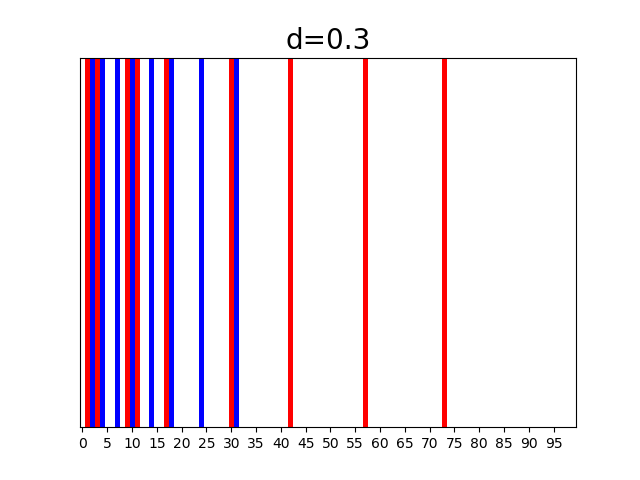
\includegraphics[width=0.2\textwidth]{images/line_line_2_0.3_eigenvector_division.png}
        \caption{Rectangle, $K=2$}
    \end{subfigure}
    \caption{The first 100 nontrivial eigenvectors of data sampled from a rectangle, separated and color-coded by manifold using varying parameters for $d$ and $K$. Each eigenvector is represented by a vertical line. Red and blue lines indicate base eigenvectors belonging to the two independent manifolds (the two lines whose product is the rectangle), and white indicates a mixture eigenvector. Within the range $[0.1, 0.2]$ over the distance threshold $d$, the results for both values of $K$ are stable.}
    \label{fig:stability_rectangle}
\end{figure}

One potential concern is that the results may be extremely sensitive to variations within a single parameter. In particular, stability over varying values of $d$ is desirable, as $d$ may vary between zero and the largest distance of any triplet. To explore this, we examine how the chosen eigenvectors compare across a range over $d$ for different fixed values of $K$. The results are shown in Figure \ref{fig:stability_rectangle}. For $K=1,2$, the predictions are stable over the range $d \in [0.1,0.2]$, but if $d$ becomes too large then the first eigenvector may be misclassified. We suspect that this is because the first eigenvector appears as a base eigenvector in the most number of triplets, and if $d$ is too large then Algorithm 1 does not sufficiently filter out unreliable triplets containing the first eigenvector, which skews the voting process.

We also ran the algorithm on the product of a rectangle and a circle, which decomposes as the product of three independent manifolds: two lines and a circle. These results are discussed in the Appendix section.

\section{Conclusion}
\subsection{Summary}
In this paper, we develop an algorithm for independent manifold analysis. One motivating application of such an algorithm is for the heterogeneity reconstruction problem in cryo-EM. Reconstructing three-dimensional models of molecules imaged by cryo-EM requires some knowledge of the manifold of possible conformations which that molecule may have. Isolating that manifold from the ambient manifold of the data can help extract this information.

Our algorithm leverages multiple spectral graph analysis techniques, including diffusion maps and spectral clustering, to analyze the Laplace eigenvectors of the data. For a large number of data points, these eigenvectors approximate the eigenfunctions of the ambient manifold. When tested on toy manifolds that are the product of two independent manifolds, it successfully distinguishes and separates the top most significant eigenvectors of either submanifold. Moreover, the predictions are stable over a reasonable range of the algorithm parameters.

\subsection{Future work}
A natural generalization for the algorithm is to handle general densities of data. The data in our experiments was randomly sampled from a uniform distribution, but this may not always be a realistic assumption. We can redefine the diffusion map in terms of the \textit{Coifman-Lafon normalized graph Laplacian} \cite{coifman2006diffusion}, which is obtained by first normalizing the weight matrix $\widetilde{W} = D^{-1}WD^{-1}$ and defining $\mathcal{L} = \widetilde{D}^{-1}\widetilde{W}$, where $\widetilde{D}$ is the degree matrix of $\widetilde{W}$. The benefit of using this variant of the graph Laplacian is that it converges to the continuous Laplacian regardless of sampling density. This approach has been shown to be effective on non-uniformly sampled data by the authors of \cite{zelesko2019earthmover}.

In future explorations, it is also necessary to have a concrete evaluation method of how well the algorithm performs on a given manifold. In order to properly evaluate the algorithm, we must have a metric which measures the algorithm's performance. In this setting, a natural metric would be to simply compare the results of the algorithm against the ground truth and count how many correct eigenvectors the algorithm chooses, while penalizing incorrect choices. These counts should also be weighted, as correctly identifying the lowest frequency (most significant) eigenvectors is an easier task than correctly identifying higher frequency ones. This is because lower frequency eigenvectors are simply considered more frequently as potential base eigenvectors, as the number of triplets in which they appear is higher. Mischaracterizing a more significant mixture eigenvector is easier than mischaracterizing a less significant eigenvector for the same reason. The difficulties of these choices also depends on the dimensionality reduction performed by the diffusion map, as this gives us greater or fewer eigenvectors to examine. A good metric should combine all of these factors.

\subsection*{Acknowledgments}
I would like to thank Dr. Amit Moscovich, Professor Amit Singer and Professor Nicolas Boumal for all their guidance and support, even through all the obstacles of this unprecedented semester.

\section{Appendix}
While the majority of our experiments were run on data sampled from two dimensional manifolds, we were also interested in how well the algorithm generalized to higher dimensional Euclidean regions. In particular, the space of possible conformations of a molecule in cryo-EM can be thought of as a rotation around a fixed axis combined with a bounded translation. In two dimensions, this would correspond to the product of a rectangle and a circle. We generated additional data consisting of 10,000 samples from the manifold $\Omega = [0, \sqrt{\pi} + 1] \times [0,1] \times [-\pi, \pi]$, and tested our algorithm on this set. The three independent intervals can be interpreted as $x \in [0, \sqrt{\pi} + 1] = \Omega_1$, $y \in [0,1] = \Omega_2$ and $\theta \in [-\pi, \pi] = \Omega_3$.

\begin{figure}[ht]
    \centering
    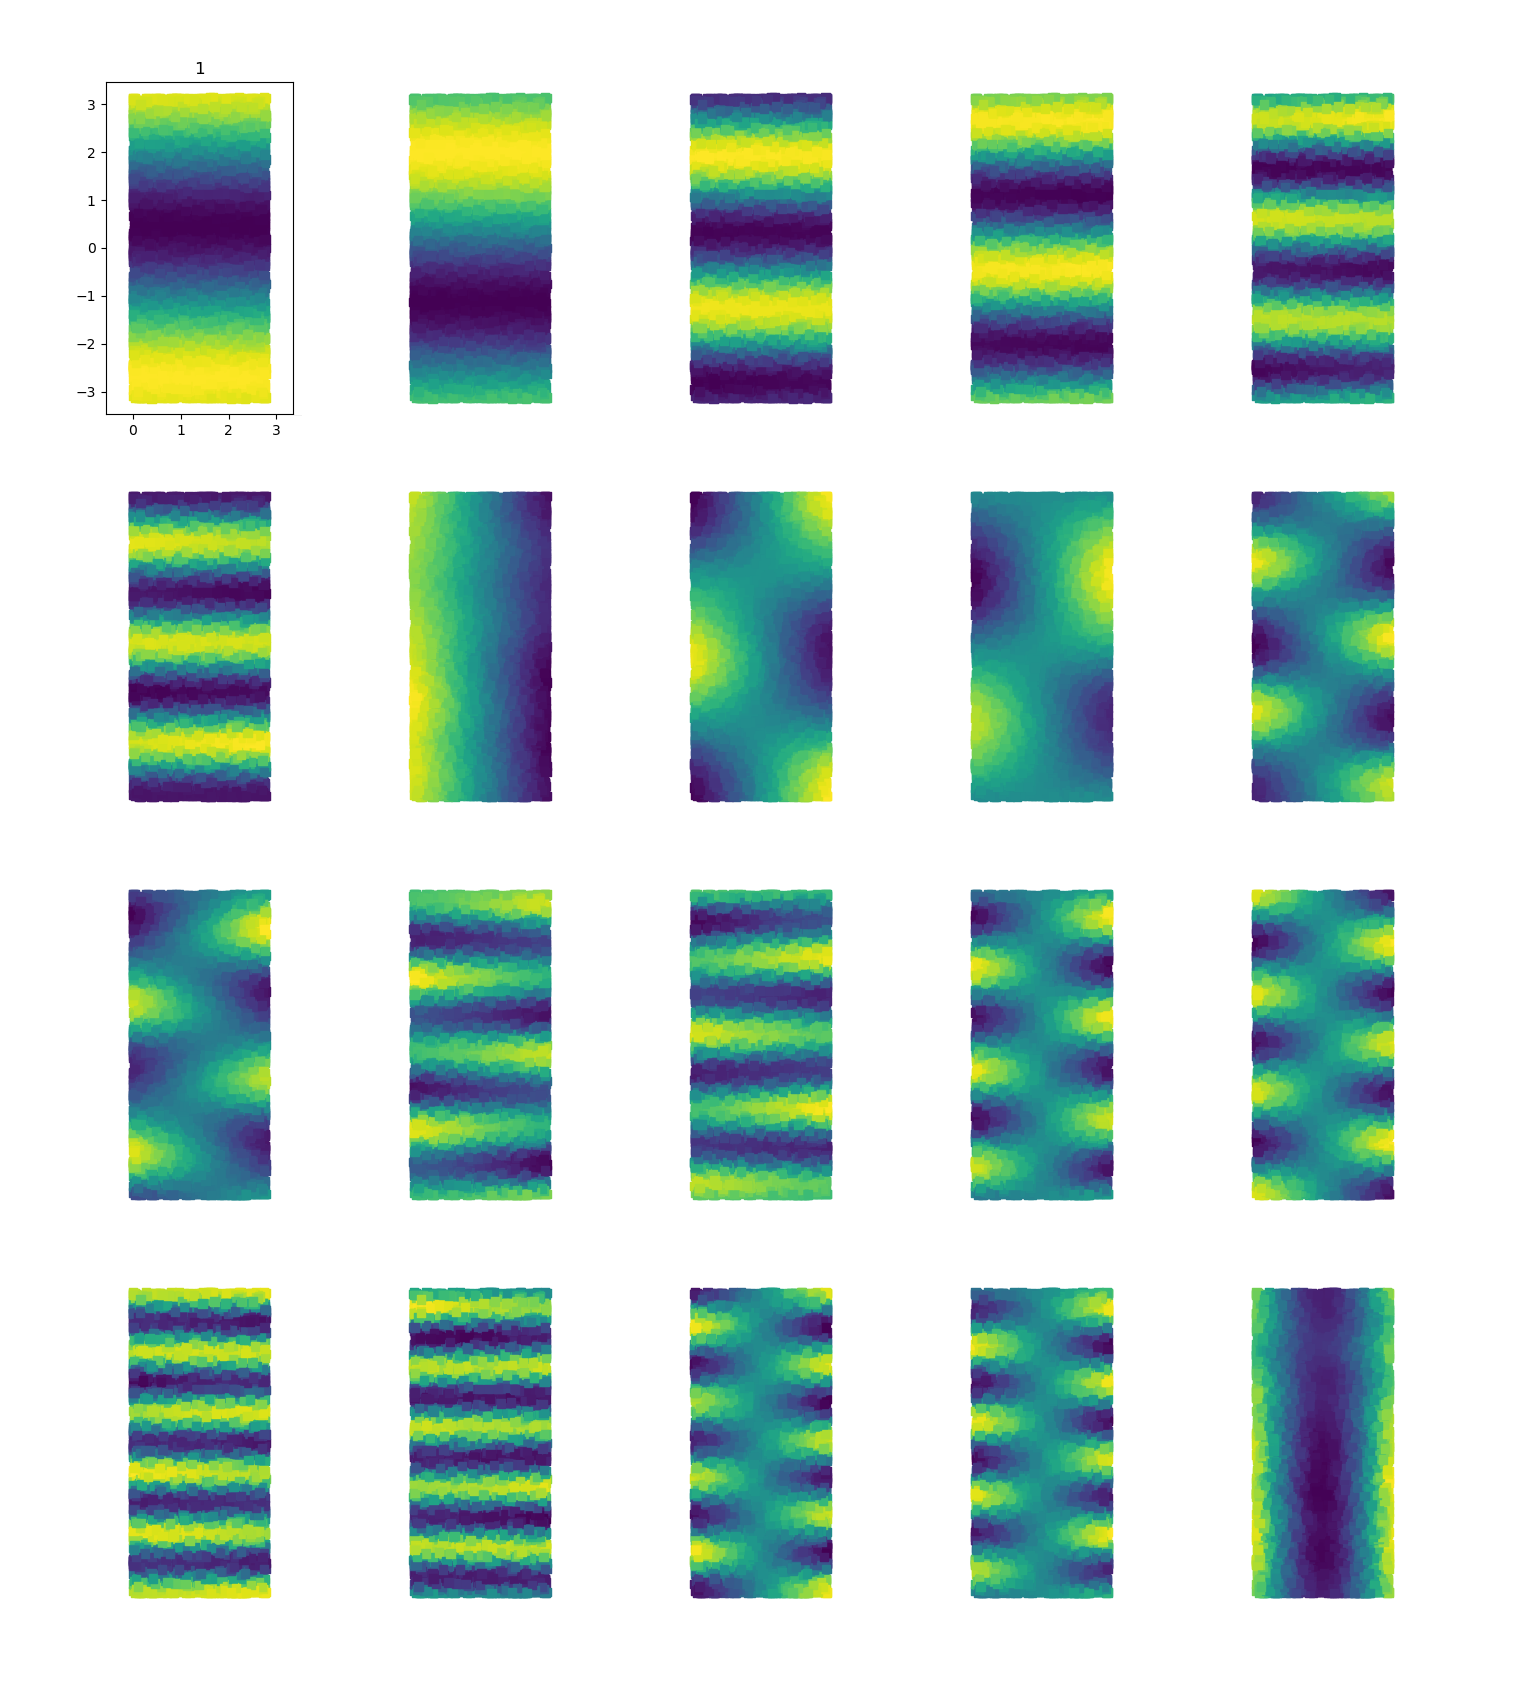
\includegraphics[width=0.56\textwidth]{images/rect_circle_eigenvalues_20_(1,3).png}
    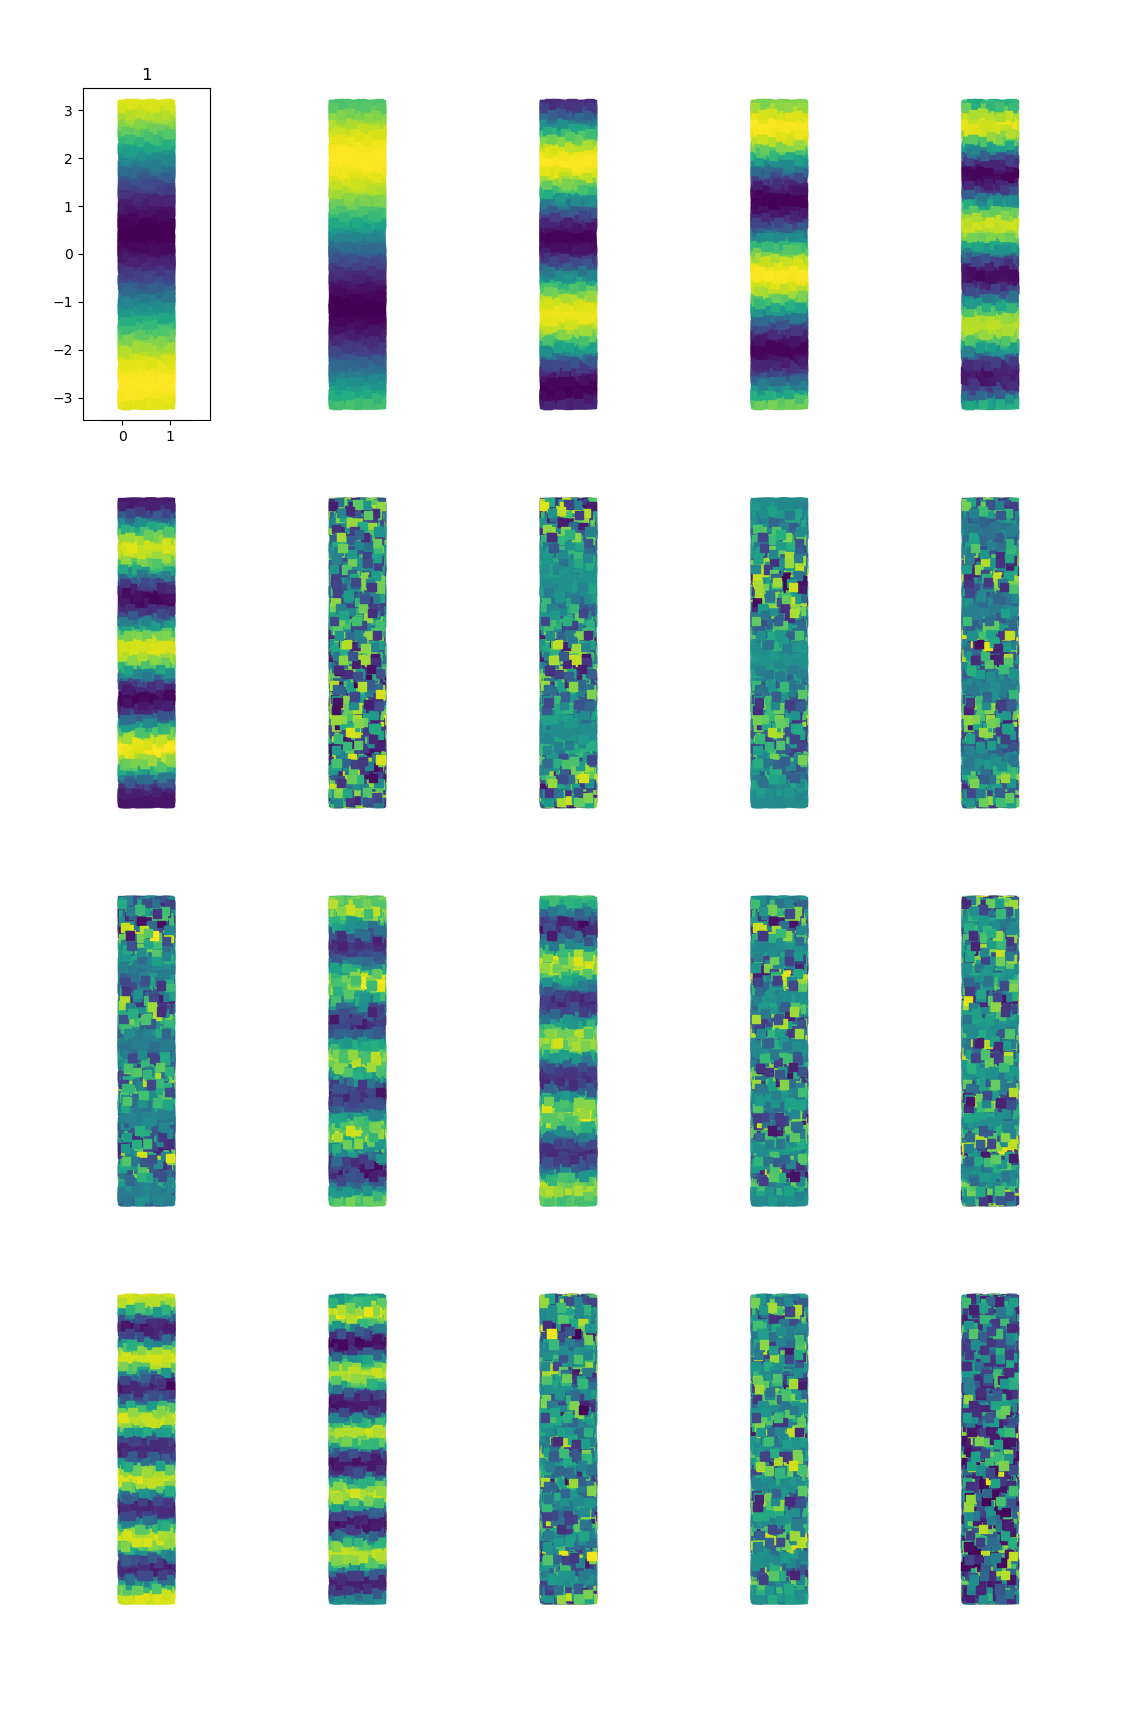
\includegraphics[width=0.42\textwidth]{images/rect_circle_eigenvalues_20_(2,3).png}
    \caption{The 20 most significant Laplace eigenvectors of 10,000 samples from the three dimensional product manifold formed $\Omega = [0, \sqrt{\pi} + 1] \times [0,1] \times [-\pi, \pi]$. The actual eigenvalues are three-dimensional, but for clarity we display them projected in the $y$-dimension (left) and in the $x$-dimension (right).}
    \label{fig:3d-all-eigenvecs}
\end{figure}

To better visualize the eigenvectors, we plot the projections of the eigenvectors in the $x$-direction and the $y$-direction. Both projections of the 20 most significant eigenvectors are shown in Figure \ref{fig:3d-all-eigenvecs}. From these visualizations we can also see which eigenvectors are mixtures of which manifolds by looking at the amount of noise in the eigenvector when projected in a certain direction. For example, the first six eigenvectors are non-noisy in both projections, so they only encode information from the $\theta$ interval and are therefore base eigenvectors of $\Omega_3$. Eigenvectors 7 through 11 appear non-noisy when projected in the $y$-direction, but noisy in the $x$-direction. We can still, however, see a sinusoidal structure to the noise, indicating that projecting in the $x$-direction removed some of the interesting information in the eigenvector, but not all of it. Thus we can conclude that these eigenvectors are mixtures of $\Omega_1$ and $\Omega_3$.

\begin{figure} 
    \centering
    \begin{subfigure}[t]{\textwidth}
        \centering
        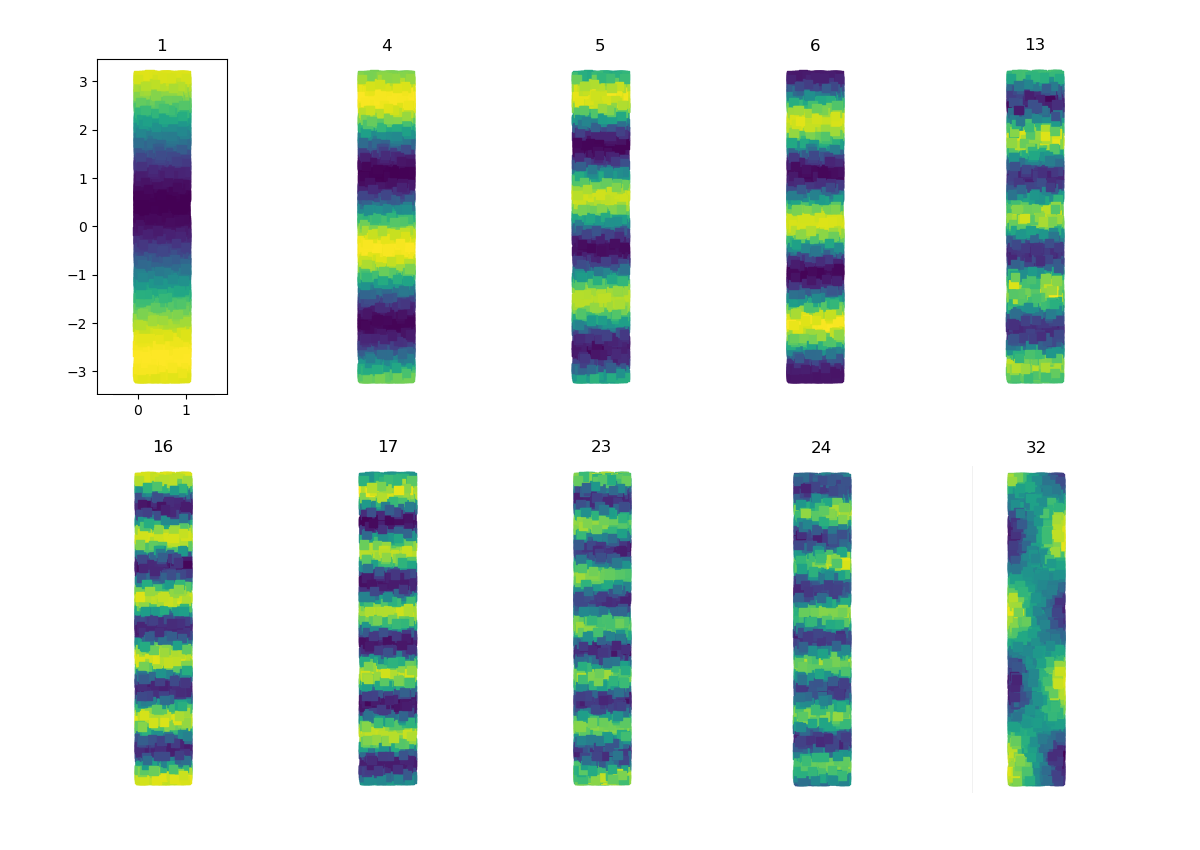
\includegraphics[width=0.71\textwidth]{images/manifold1_rect_circle_(2,3).png}
        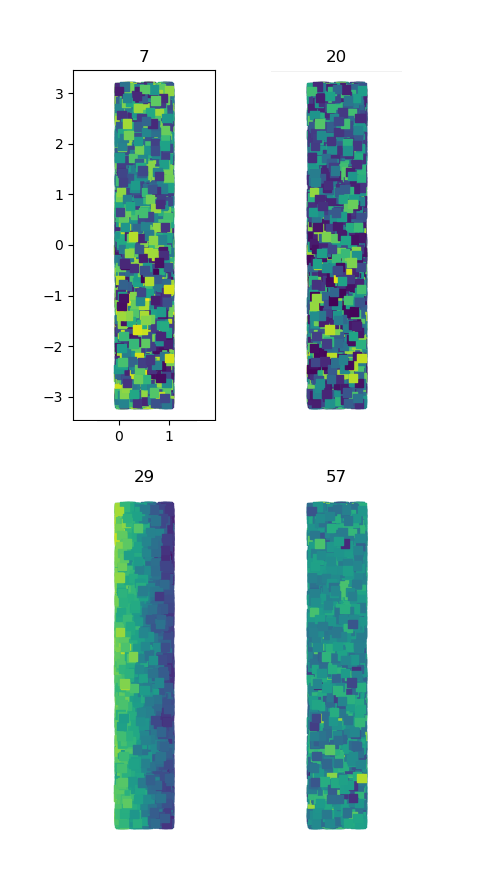
\includegraphics[width=0.28\textwidth]{images/manifold2_rect_circle_(2,3).png}
        \caption{Separated eigenvectors projected in the $x$-direction.}
    \end{subfigure}
    \begin{subfigure}[t]{\textwidth}
        \centering
        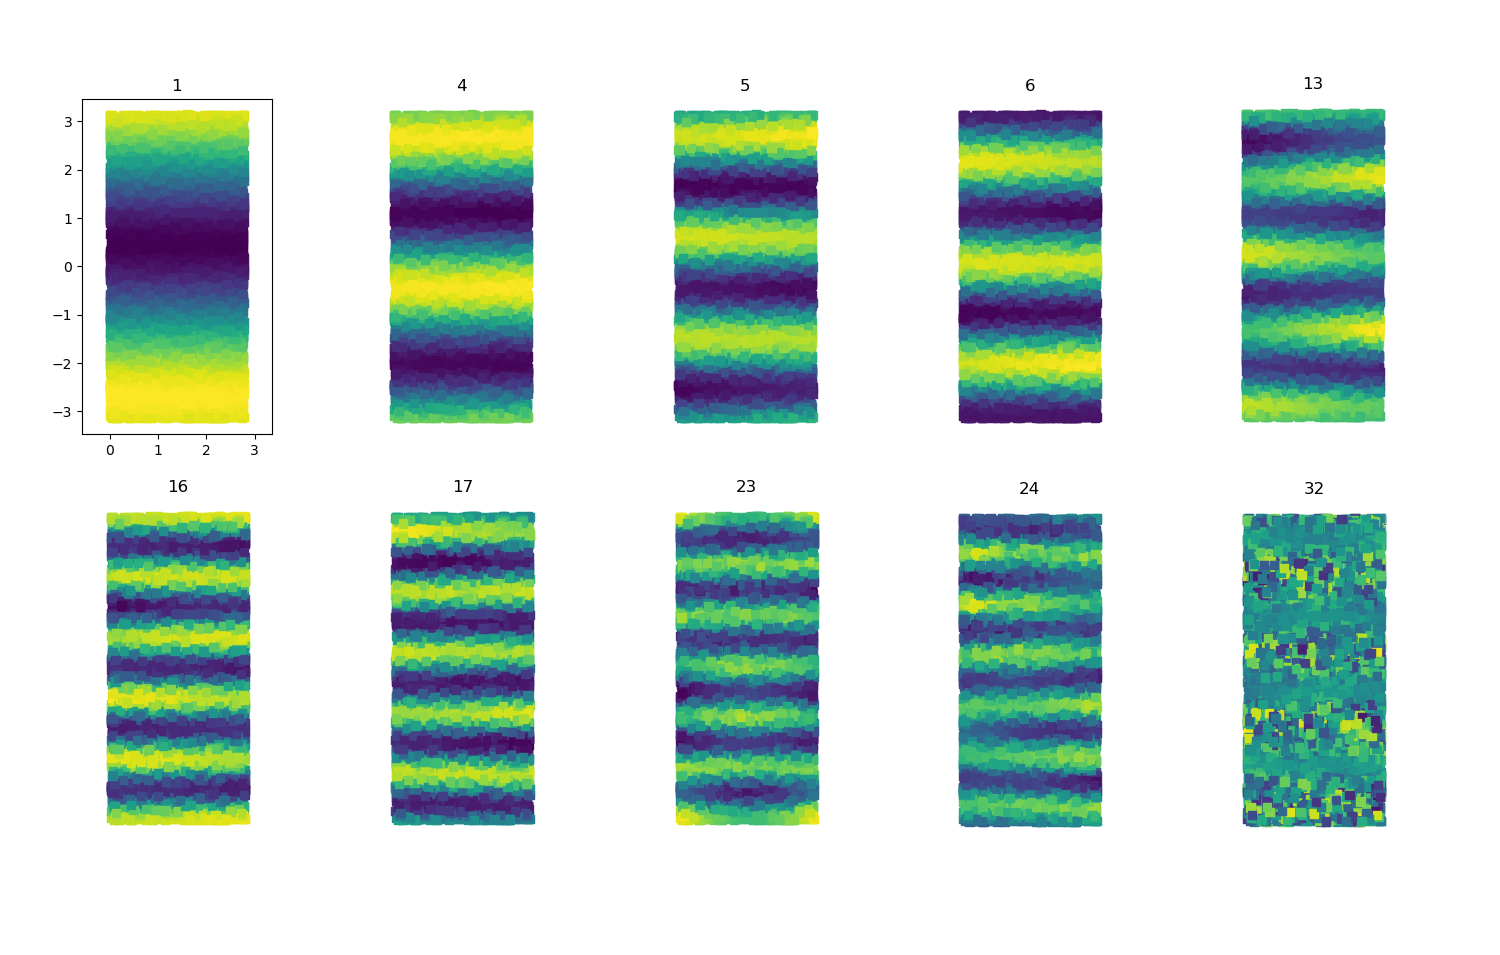
\includegraphics[width=0.65\textwidth]{images/manifold1_rect_circle_(1,3).png}
        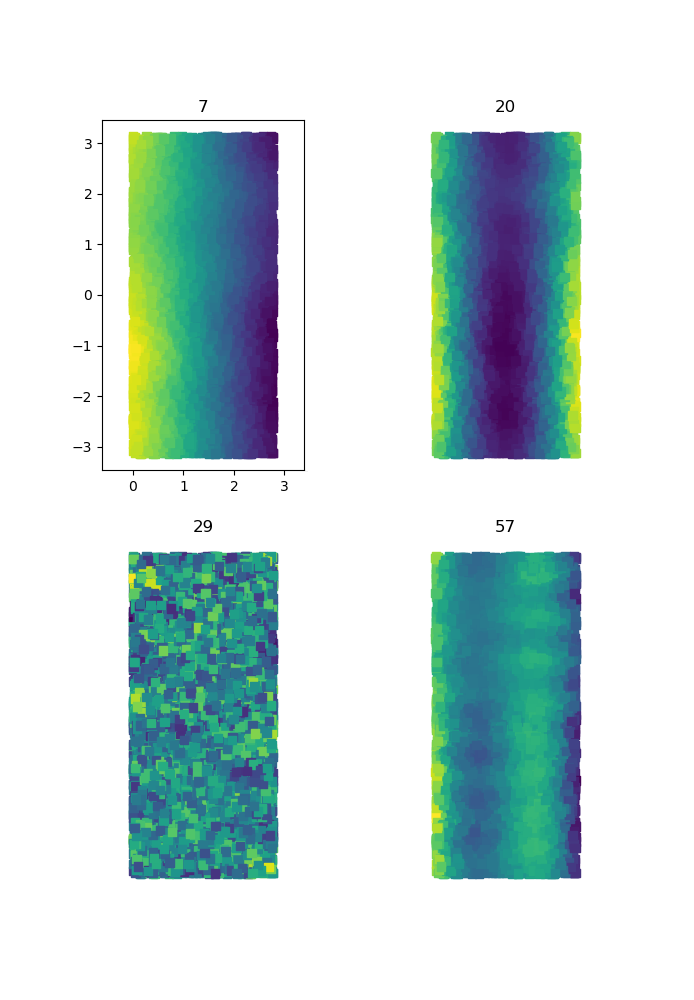
\includegraphics[width=0.29\textwidth]{images/manifold2_rect_circle_(1,3).png}
        \caption{Separated eigenvectors projected in the $y$-directions.}
    \end{subfigure}
    \caption{Separated eigenvectors projected in (a) the $x$-direction and (b) the $y$-direction. One group contains eight eigenvectors (on the left) while the other contains four (on the right). Notice how in (a), only one eigenvector on the right does not appear noisy. This indicates that this group of eigenvectors can be decomposed further. In (b), the same eigenvector is noisy while the others are non-noisy. This indicates that the group of eigenvectors on the right can be decomposed further.}
    \label{fig:3d-2groups}
\end{figure}

\begin{figure} 
    \centering
    \begin{subfigure}[t]{\textwidth}
        \centering
        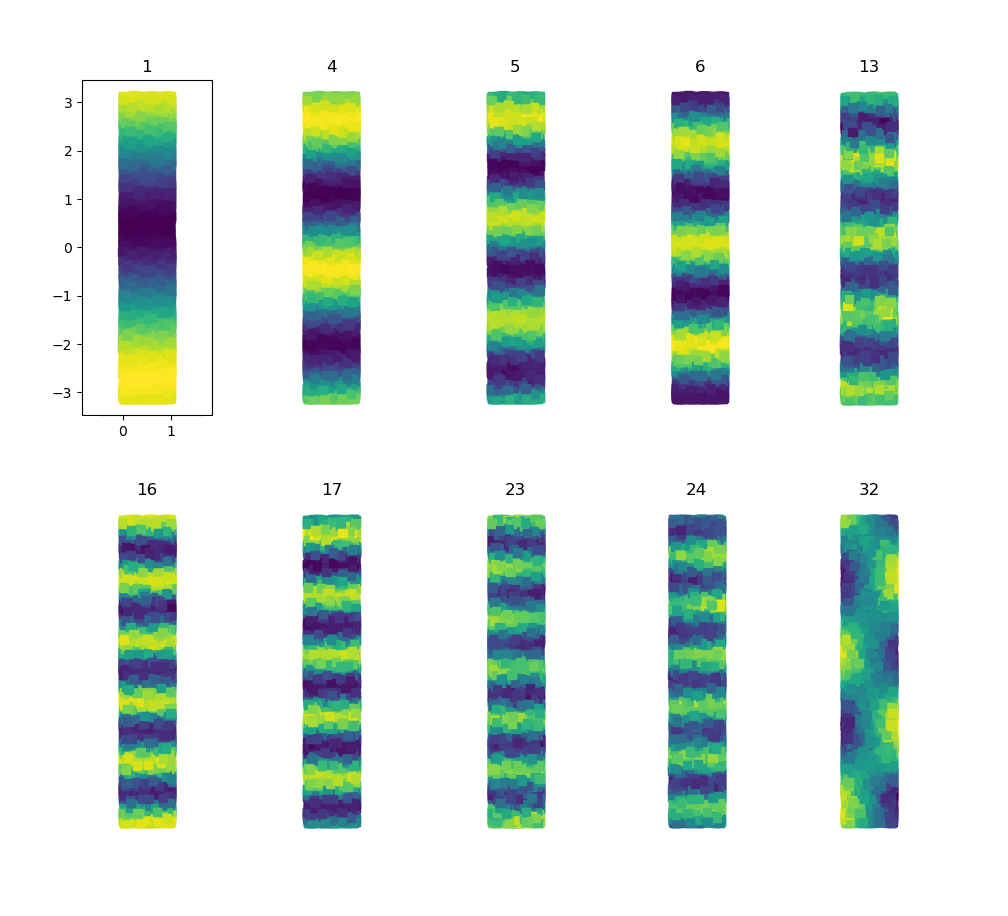
\includegraphics[width=0.41\textwidth]{images/manifold1_rect_circleA.png}
        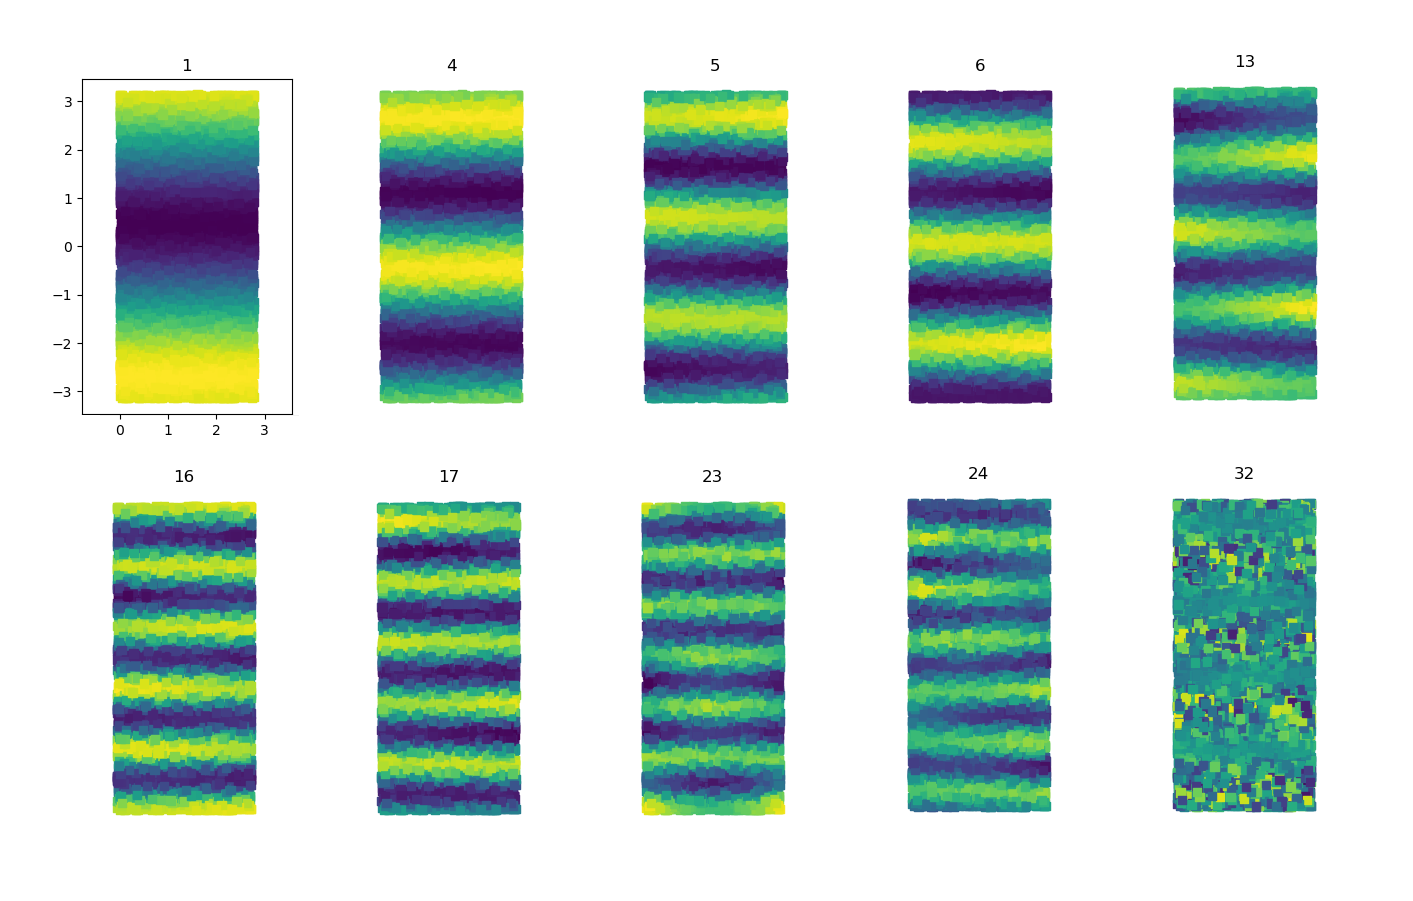
\includegraphics[width=0.58\textwidth]{images/manifold1_rect_circleB.png}
        \caption{Base eigenvectors associated with $\Omega_3$ (the $\theta$ variable), projected in the $x$-direction (left) and in the $y$-direction (right).}
    \end{subfigure}
    \begin{subfigure}[t]{\textwidth}
        \centering
        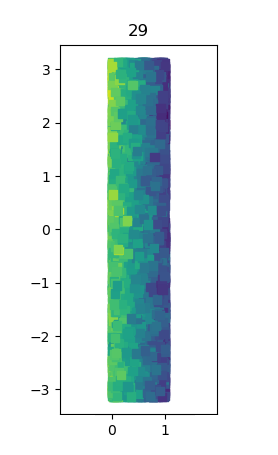
\includegraphics[width=0.24\textwidth]{images/manifold2_rect_circle.png}
        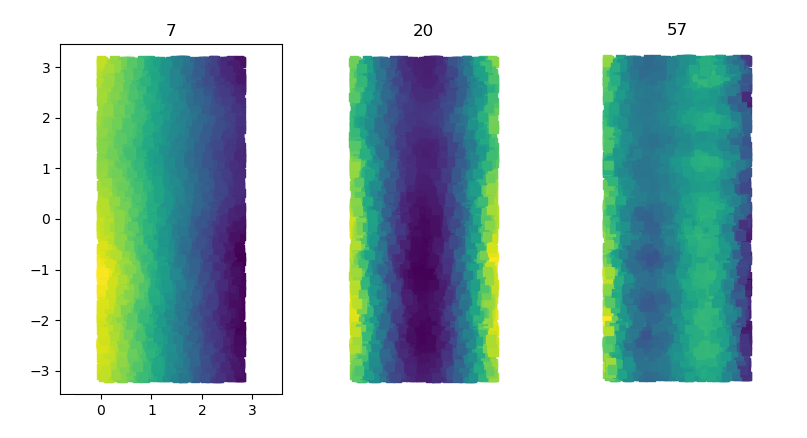
\includegraphics[width=0.74\textwidth]{images/manifold3_rect_circle.png}
        \caption{Base eigenvectors associated with $\Omega_1$ (the $x$ variable), projected in the $y$-direction (left) and base eigenvectors associated with $\Omega_2$ (the $y$ variable), projected in the $x$-direction (right).}
    \end{subfigure}
    \caption{The base eigenvectors of the product of two lines and a circle, separated into three groups by the algorithm. Notice how the last eigenvector in (a) appears noisy on the right image. This not only indicates that it was incorrectly chosen, but also that it is a mixture eigenvector of exactly $\Omega_2$ and $\Omega_3$. The bottom left image corresponds to the base eigenvector of $\Omega_2$, and the bottom right image corresponds to the base eigenvectors of $\Omega_1$. All of the eigenvectors chosen are base eigenvectors except for the aforementioned one in (a).}
    \label{fig:3d-3groups}
\end{figure}

Using the parameters $d = 0.17$, $K = 2$, running the algorithm to separate the eigenvectors into two groups produces the separations shown in Figure \ref{fig:3d-2groups}. The projected views show that the clusters align well with the rectangle and circle decomposition. We can also run the algorithm to separate the eigenvectors into three groups, by using spectral clustering with three clusters instead of two. The results are shown in Figure \ref{fig:3d-3groups}. This produces an even better decomposition, preserving the group of base  eigenvectors associated with $\Omega_3$ but separating the other eigenvectors into their respective manifolds $\Omega_1$ or $\Omega_2$. This shows that the algorithm is viable for decomposing manifolds of higher dimensions.

\clearpage
\addcontentsline{toc}{section}{References}
\bibliography{refs}

\end{document}
